%===============================================================================
% Template Name:      SUnORE Starter Presentation template
% Template URI:       http://sunore.co.za/sunore-presentation/
% Description:        Starter Presentation template for SUnORE 
%                     Department of Industrial Engineering, 
%                     Stellenbosch University
% Version:            1.1.0
% Author:             Johan Janse van Rensburg
% Author URI:         http://johanjvrens.co.za/
% License:            MIT License
% License URI:        http://opensource.org/licenses/MIT
%===============================================================================
\documentclass[serif,11pt]{beamer}

%=================================================
% theme and color
%=================================================
\usetheme{Warsaw} %Themes http://www.hartwork.org/beamer-theme-matrix/
\definecolor{colorA}{RGB}{96, 34, 59}
\definecolor{colorB}{RGB}{140, 151, 154}
%\definecolor{secinhead}{RGB}{249,196,95}
%\definecolor{titlebg}{RGB}{51,51,51}
\setbeamercolor{structure}{fg=colorA,bg=colorB}
%\setbeamercolor{secsubsec}{fg=secinhead,bg=black}
%\setbeamercolor{frametitle}{fg=secinhead,bg=titlebg}

%=================================================
% packages and new commands
%=================================================
\usepackage[ruled, linesnumbered, vlined]{algorithm2e}
\usepackage{epsfig, subfigure, amssymb, multirow, algorithmic, amsmath}
\newcommand*{\superscript}[1]{\ensuremath{^{\rm #1}}}
\newcommand*{\subscript}[1]{\ensuremath{_{\rm #1}}}
\usepackage{amstext}
\usepackage{amscd}
\usepackage{amsthm}
\usepackage{amsbsy}
\usepackage{amssymb}
\usepackage{appendix}
\usepackage{enumerate}
\usepackage{multirow}
\usepackage[mathscr]{eucal}
\usepackage{fancyhdr}
\usepackage{supertabular}
\usepackage{fancybox}
\usepackage{array}
\usepackage{booktabs}
\usepackage{soul}
\usepackage{epic}
\usepackage{float}
\usepackage{appendix}
\usepackage{hyperref}
%=================================================
% thesis details (preamble)
%=================================================
\title[{\sc Numerical Solutions for Burgers’ Equation } \hspace{0.8cm} \insertframenumber/\inserttotalframenumber]{{\sc Numerical Solutions for Burgers’ Equation in the Stochastic and Deterministic Version Using Spectral Methods }}
\author[Presentacion de Examen de Grado --- {\sc Sep 18\superscript{th}, 2020}]{{Alan Daniel Matzumiya Zazueta}}
\date{18 Sep 2020}
\institute{Universidad de Sonora \\ Division de Ciencias Exactas y Naturales \\ Programa de Posgrado en Matematicas}
%=================================================
% start presentation
%=================================================
\begin{document}
%========================
% title page
%========================
\begin{frame}
  \begin{center}
    
\includegraphics[scale=0.13]{files/logo.png}
  \end{center}
  \titlepage
\end{frame}
%========================
% your slides:
%========================
\label{Contenido}
\begin{frame}{Contenido \hspace{7cm} \hyperlink{Navegador}{\beamergotobutton{Navegador}}}
	\begin{itemize}
		\only<1->{
		\item Motivación y Objetivos. \hyperlink{Motivación y Objetivos}{\beamergotobutton{Ir}}
		}
		\vspace{1mm}
		\only<2->{
		\item Soluciones de la Ecuación de Burgers' Determinista.
		}
		\vspace{1mm}
		\only<3->{ 
    	\begin{itemize}
		    \vspace{1mm}
    		\item Método de Fourier-Galerkin: Operador Proyección. \hyperlink{Proyección}{\beamergotobutton{Ir}} 
		    \vspace{1mm}	
    		\item Método de Fourier-Colocación: Operador Interpolación. \hyperlink{Interpolación}{\beamergotobutton{Ir}} 
    	\end{itemize}	
    	}
		\vspace{1mm}
		\only<4->{
		\item Soluciones de la Ecuación de Burgers' Estocástica.
		}
		\vspace{1mm}
		\only<5->{
		\begin{itemize}
    		\item Relación Entre la Ecuación de Fokker-Planck-Kolmogorov (FPK). \hyperlink{FPK}{\beamergotobutton{Ir}} 
		    \vspace{1mm}    
    		\item Solución Numérica Asociada a la Ecuación de (FPK). \hyperlink{Estocástica}{\beamergotobutton{Ir}} 
    	\end{itemize}
		}
		\vspace{1mm}
		\only<6->{
		\item Discusión y Conclusiones. \hyperlink{Conclusiones}{\beamergotobutton{Ir}} 
		}
	\end{itemize}
\end{frame}
\label{Motivacion y Objetivos}
\begin{frame}{\hyperlink{Navegador}{\beamergotobutton{Navegador}}}
    \begin{block}{Motivación}
    \begin{itemize}
		\only<1->{
		\item La importancia de estudiar ecuaciones diferenciales. 
		}
		\only<2->{
		\item Contar con herramientas adecuadas para su estudio.
		}
		\only<3->{
		\item En dinámica de fluidos computacionales, los métodos espectrales son una alternativa viable.
		}
		\only<4->{
		\item Además, fáciles de implementar y poder profundizar el estudio de esta área.
		}
    \end{itemize}
    \end{block}
\end{frame}

\begin{frame}{\hyperlink{Navegador}{\beamergotobutton{Navegador}}}
    \begin{block}{Objetivos}
    \begin{itemize}
        \only<1->{
        \item Comprender los fundamentos de los métodos espectrales.
        }
        \only<2->{
		\item Implementarlos en la ecuación de Burgers' Determinista. 
		}
		\only<3->{
		\item Hacer un análisis cualitativo detallado de las soluciones obtenidas.
		}
		\only<4->{
		\item Resolver la versión estocástica usando un método espectral. 
		}
		\only<5->{
		\item Evaluar y argumentar los resultados obtenidos con estos métodos. 
		}
	\end{itemize}
	\end{block}
\end{frame}
\label{Proyeccion}
\begin{frame}{Operador Proyección \hspace{5cm} \hyperlink{Navegador}{\beamergotobutton{Navegador}}}
    \only<1->{
    \begin{block}{Expansión de Fourier}
    		\begin{equation*}  
    		    F[u] \equiv \displaystyle \sum_{ |n| \leq \infty} \hat{u}_{n} e^{inx}.
    		\end{equation*}
    \end{block}
    }
    \only<2->{
	\begin{block}{Coeficientes de Fourier}
    	\begin{equation*}
    	    \hat{u}_n = \frac{1}{2 \pi} \displaystyle \int_{0}^{2 \pi} u(x) e^{-inx} dx, \hspace{3mm}  k = 0, \pm 1, \pm 2, \dots, \hspace{2mm} u(x) \in L^2 [0, 2 \pi].
    	\end{equation*}
	\end{block}
	}
	\only<3->{
    \begin{block}{Expansión Truncada: Proyección}
    	\begin{equation*}
    	u_N (x, t) = \displaystyle \sum_{ |n| \leq \frac{N}{2} } \hat{u}_n e^{inx} 
    	\end{equation*}
    \end{block}	
    	}
\end{frame}
\label{Determinista}
\begin{frame}{Ecuación de Burgers' Determinista \hspace{2cm} \hyperlink{Navegador}{\beamergotobutton{Navegador}}}
	\only<1->{
	\begin{block}{Ecuación de Burgers'}
    \begin{equation*}
        \left \lbrace \begin{array}{ll}
    	u_t + u u_x = \alpha u_{xx} & x \in \mathbb{R}, \hspace{2mm} t > 0, \hspace{2mm} \alpha \geq 0 \\
    	u (x, 0) = u_0 (x)  & x \in \mathbb{R},
    	\end{array}  \right .
    \end{equation*}
    \end{block}
    }
    \only<2->{
    \begin{block}{Ecuación de Difusión}
    \begin{equation*}
        \left \lbrace \begin{array}{ll}
    	\varphi_t - \alpha \varphi_{xx} = 0,  & x \in \mathbb{R}, \hspace{2mm} t > 0, \hspace{2mm} \alpha > 0, \\
    	\varphi (x, 0) = \varphi_0 (x) = \displaystyle e^{- \int_{0}^{x} \frac{u_0 (y)}{2 \alpha} dy}, & x \in \mathbb{R}.
    	\end{array}  \right .
    \label{heat}
    \end{equation*}
    \end{block}
    }
    \only<3->{
    \begin{block}{Solución Analítica: Transformación de Cole-Hopf}
    \begin{equation*}
        u (x, t) = -2 \alpha \frac{\varphi_x}{\varphi} =  \displaystyle \frac{\int_{-\infty}^{\infty} \frac{x - \xi}{t} \varphi_0 (\xi) e^{- \frac{(x - \xi)^2}{4 \alpha t}} d\xi}{\int_{-\infty}^{\infty} \varphi_0 (\xi) e^{- \frac{(x - \xi)^2}{4 \alpha t}} d\xi} 
    \end{equation*}
    \end{block}
    }
\end{frame}    

\label{Galerkin}
\begin{frame}{Método de Fourier-Galerkin \hspace{4cm} \hyperlink{Navegador}{\beamergotobutton{Navegador}}}
    \only<1->{	
    \begin{block}{Fourier-Galerkin}
		\begin{align*}
    	\left \langle \frac{\partial u_N}{\partial t} - \alpha \frac{\partial^2 u_N}{\partial x^2} + \frac{1}{2} (u_N^2)_x, e^{inx} \right\rangle = 0, \hspace{2mm} \forall \hspace{2mm} |n| \leq N, \hspace{2mm} \forall t > 0 \\
    	\left \langle \frac{\partial \varphi_N}{\partial t} - \alpha \frac{\partial^2 \varphi_N}{\partial x^2}, e^{inx} \right\rangle = 0, \hspace{2mm} \forall \hspace{2mm} |n| \leq N, \hspace{2mm} \forall t > 0
		\end{align*}
	\end{block}
	}
	\only<2->{
	\begin{block}{Sistema de EDOs}
	\begin{align*}
	    \frac{d \hat{u}_n (t)}{dt} &= \alpha p^2 n^2 \hat{u}_n (t) - p \widehat{G}_n (t) , \hspace{0.3cm} \forall |n| \leq \frac{N}{2} \\
    	u_N(0) &= \mathcal{P}_N u_0 (x) \\ 
	    \frac{d \hat{\varphi}_n (t)}{dt} &= - \alpha P^2 n^2 \hat{\varphi}_n (t), \hspace{2mm} |n| \leq N \\
    	\varphi_N (0) &= \mathcal{P}_N \varphi_0 (x)
	\end{align*}
	\end{block}
	}
\end{frame}

\label{Solucion-Galerkin}
\begin{frame}{Solucion Numerica: Fourier-Galerkin \hspace{2cm} \hyperlink{Navegador}{\beamergotobutton{Navegador}}}
	\only<1->{
	\begin{block}{Solucion Numerica: Discretizaci\'on Semi-Impl\'icita}
	Para $\Delta t \in \mathbb{R}$ y $M \in \mathbb{N}$ fijos,  $t_j = j \Delta t, \hspace{2mm} j = 0, 1, \dots, M$ definimos:
	\begin{align*}
	\hat{u}_n (t_{j+1}) = \hat{u}_n (t_j) &+ \Delta t \alpha p^2 n^2 \hat{u}_n (t_j)	\\
	&- in p \Delta t \displaystyle \left( \sum_{|k| \leq \frac {N}{2}} \hat{u}_n (t_{j+1}) \hat{u}_{n - k} (t_{j+1}) \right)
	\end{align*}
	\end{block}
	}
	\only<2->{
	\begin{block}{Solucion Analitica Aproximada}
	\begin{equation*}
		u_N (x, t)  = - 2 \alpha \frac{\partial_x \varphi_N (x, t)}{ \varphi_N (x, t)} = - 2 \alpha \frac{\displaystyle \sum_{ |n| \leq N} in \hat{\varphi}_n (0) e^{- \lambda_n t}  \phi_n (x) }{\displaystyle \sum_{|n| \leq N} \hat{\varphi}_n (0) e^{- \lambda_n t}  \phi_n (x)}
	\end{equation*}
	\end{block}
	}
\end{frame}

\begin{frame}{Simulaciones: Fourier-Galerkin \hspace{2.5cm} \hyperlink{Navegador}{\beamergotobutton{Navegador}}}
	\only<1->{	
	Para los siguientes resultados numericos se considero lo siguiente	
	\begin{equation*}
		u_0 (x) = e^{-0.05 x^2}, \hspace{3mm} x \in [-60, 60], \hspace{2mm} t \in [0, 100]. 
	\end{equation*}
	}
\end{frame}

\label{Cero-Viscosidad}
\begin{frame}{Ecuacion de Burgers': Sin Viscosidad \hspace{1cm} \hyperlink{Navegador}{\beamergotobutton{Navegador}}}
	\begin{align*}
		u(x, t) &= u_0 (x_0), \hspace{2mm} x_0 = x - u_0 (x_0) t, \hspace{2mm} t \in [0, T_c], \\
		u_0 (x) &= e^{-0.005 x^2}, \hspace{3mm} x \in [-60, 60], Tc = \min_{x \in \mathbb{R}} \left[  \frac{-1}{u'_0 (x)} \right], 
	\end{align*}
\end{frame}
\label{Interpolacion}
\begin{frame}{Operador Interpolacion \hspace{5cm} \hyperlink{Navegador}{\beamergotobutton{Navegador}}}
    \only<1->{
    \begin{block}{Puntos de Colocacion}
    \begin{align*}
        x_j = \frac{2 \pi}{N + 1} j , \hspace{0.5cm} j\in [0, \dots , N],
    \end{align*}
    \end{block}
    }
    \only<2->{
    \begin{block}{Aproximacion de Coeficientes: Regla del Trapecio}
    \begin{align*}
        \hat{u}_n \approx \widetilde{u}_n = \frac{1}{N + 1} \displaystyle \sum_{j = 0}^{N} u(x_j) e^{-in x_j}
    \end{align*}    
    \end{block}
    }
    \only<3->{
    \begin{block}{Interpolador}
    Para cada $j \in [ 0, \dots , N ]$ satisface $\mathcal{J}_N u (x_j) =  u (x_j)$, y
    \begin{align*}
        \mathcal{J}_N u(x) =  \displaystyle \sum_{ |n| \leq \frac {N}{2}} \widetilde{u}_n e^{inx}
	\end{align*}
	\end{block}
	}
\end{frame}

\label{Colocacion}
\begin{frame}{Metodo de Fourier-Colocacion \hspace{3cm} \hyperlink{Navegador}{\beamergotobutton{Navegador}}}
	\only<1->{
	\begin{block}{Fourier-Colocacion}
	Para cada $j = 0, 1, \dots, 2N$, $t \geq 0$ configurarmos 
	$u_N (t) = [u_N (x_i , t), u_N (x_1 , t), \dots, u_N (x_{2N} , t]^T$, $u_N (0) =  u_0$, y debe satisfacer,
	\begin{align*}
		\left\langle \frac{\partial u_N}{\partial t} - \alpha \frac{\partial^2 u_N}{\partial x^2} + \frac{1}{2} \mathcal{J}_N (u_N^2)_x, \phi \right\rangle_N = 0, \hspace{2mm} t > 0, \hspace{2mm}
	\end{align*}
	Equivalentemente,
	\begin{align*}
		\frac{d u_N (t)}{dt} =  \alpha D_N^2 u_N (t) - \frac{1}{2} D_N u^2_N (t), 
	\end{align*}
	\end{block}
	}
	\only<3->{
	\begin{block}{Matriz de Diferenciacion}
	\begin{align*}
	    \widetilde{D}_{ij} = -\delta_{ij} \frac{(-1)^{i+j}}{2} \left[\sin \left[ \frac{x_i - x_j}{2}\right]\right]^{-2}, D^2_N = D_N \dot D_N
	\end{align*}
	\end{block}
	}
\end{frame}
\label{Solucion-Colocacion}
\begin{frame}{Solucion Numerica: Colocacion \hspace{3cm} \hyperlink{Navegador}{\beamergotobutton{Navegador}}}
	\only<1->{
	\begin{block}{Solucion Numerica: Discretizacion Semi-Implicita}
    	Para $\Delta t \in \mathbb{R}$ y $M \in \mathbb{N}$ fijos,  $t_j = j \Delta t, \hspace{2mm} j = 0, 1, \dots, M$ definimos:
	    \begin{align*}
		u_N (t_{i + 1} ) =  \displaystyle \left[I_N + \frac{\Delta t}{2} u_{0} \Lambda_N \right]^{-1} e^{-\Delta t \Lambda^0_N} \left[ u_N (t_{i})  - \frac{\Delta t}{2} D_N u^2_N (t_{i}) \right]
	\end{align*}
	\end{block}
	}
\end{frame}

\begin{frame}{Simulacion: Colocacion \hspace{5cm} \hyperlink{Navegador}{\beamergotobutton{Navegador}}}
    \only<1->{
	\begin{block}{Configuracion del Problema.  \hyperlink{Figuras-Colocacion}{\beamergotobutton{Simulaciones}}}
	Para los siguientes resultados numericos se considero lo siguiente	
	\begin{equation*}
		u_0 (x) = e^{-0.05 x^2}, \hspace{3mm} x \in [-60, 60], \hspace{2mm} t \in [0, 100]. 
	\end{equation*}
	\end{block}
	}
\end{frame}
\label{FPK}
\begin{frame}{Ecuacion de Fokker-Planck-Kolmogorov (FPK) \hyperlink{Navegador}{\beamergotobutton{Navegador}}}
	\only<1->{
	\begin{block}{Ecuacion de Kolmogorov}
    	\begin{equation*}
    		\frac{\partial u}{\partial t} = \frac{1}{2} Tr(QD^2 u) + \langle Ax, Du\rangle_{\mathcal{H}} + \langle B(x), Du\rangle_{\mathcal{H}}, \hspace{0.1cm} x \in D(A)
    	\end{equation*}
	\end{block}
	}
	\only<2->{
	\begin{block}{Ecuacion Estocastica. Ruido: Proceso de Wiener}
	\begin{align*}
		dX &= [AX + B(X)]dt + dW_t \\
		X(0) &= x, \hspace{0.2cm} x \in \mathcal{H}
	\end{align*}
	\end{block}
	}
	\only<3->{
	\begin{block}{Solucion de Kolmogorov: Asociacion}
	\begin{equation*}
		u(x, t) = \mathbb{E} \left[ u_0 (X^x_t) \right], 
	\end{equation*}
	\end{block}
	}
\end{frame}

\begin{frame}{Aproximacion de la Ecuacion de FPK \hspace{1cm} \hyperlink{Navegador}{\beamergotobutton{Navegador}}}
	\only<1->{
	La solucion espectral esta dada como
	\begin{block}{Expansion de Wienner-Chaos: Polnomios de Hermite}
	\begin{align*}
		u(t, x) = \displaystyle \sum _{n \in \mathcal{J}} u_{n}(t) H_n (x), \hspace{0.1cm} x \in \mathcal{H}, \hspace{0.1cm} t \in [0, T],
	\end{align*}		
	\end{block}
	}
	\only<2->{
	substituyendo en la ecuacion de Kolmogorov
	\begin{block}{Aproximacion}
	\begin{equation*}
		\dot{u}_{m} (t) = -u_{m} (t) \lambda_{m} + \displaystyle \sum _{n \in \mathcal{J}} u_{n} (t) C_{n, m} , \hspace{0.1cm} n, m \in \mathcal{J}
	\end{equation*}
	\begin{equation*}
		\mathcal{J} = \{\alpha = (\alpha_i,i \geq 1) | \alpha_i \in \mathbb{N}\cup \{0\}, |\alpha|:= \displaystyle \sum _{i = 0}^{\infty}\alpha_i < \infty\}
	\end{equation*}
	\end{block}
	}
\end{frame}
\label{Estocastica}
\begin{frame}{Ecuacion de Burgers' Estocastica \hspace{1cm} \hyperlink{Navegador}{\beamergotobutton{Navegador}}}
\only<1->{
	\begin{block}{Ecuacion de Burgers' Estocastica}
	\begin{equation*}
		d X(\xi, t) = \left[\alpha \partial_{\xi}^2 X(\xi, t) + \frac{1}{2} \partial_\xi \left(X^2 (\xi, t)\right) \right] dt + dW_t (\xi, t), \hspace{0.2cm} \xi \in [0, 1] 
	\end{equation*}
	\begin{align*}
		X(0, t) &= X(1, t) = 0 , \hspace{2mm} t > 0, \\
		X(\xi, 0) &= x(\xi), \hspace{2mm}  x \in \mathcal{H},
	\end{align*}
	\end{block}
	}
	\only<2->{
	\begin{block}{Conjunto de Indices}
	\begin{equation*}
		J^{M, N} = \{\gamma = (\gamma_i, \hspace{1mm} 1 \leq i \leq M  ) \hspace{1mm} | \hspace{1mm} \gamma_i \in \{0, 1, \cdots, N \} \}
	\end{equation*}
	\end{block}
	}
	\only<3->{
	\begin{block}{Expansion Truncada}
	\begin{equation*}
		\hat{u}_N (x, t) = \displaystyle \sum_{ n \in J^{M, N} } u_n (t) H_n (x), \hspace{2mm} x \in \mathcal{H}, \hspace{2mm}, t \in [0, T].
	\end{equation*}
	\end{block}
	}
\end{frame}

\begin{frame}{Ecuacion de Burgers' Estocastica \hspace{1cm} \hyperlink{Navegador}{\beamergotobutton{Navegador}}}
    \only<1->{
	\begin{block}{Sistema de ODEs}
	\begin{equation*}
		\dot{u}_{m} (t) = -u_{m} (t) \lambda_{m} + \displaystyle \sum _{n \in S_N} u_{n} (t) \bar{C}_{n, m} , \hspace{0.1cm} n, m \in S_N
	\end{equation*}
	\end{block}    
	}
	\begin{block}{Forma Vectorial}
	\begin{equation*}
		U^M (t) =
		\begin{pmatrix}
		u_{m_1} (t) & u_{m_2} (t) & \dots & u_{m_M} (t)
		\end{pmatrix}^T   
	\end{equation*}
	\begin{equation*}
		\dot{U}^M (t) =
		\begin{pmatrix}
		\dot{u}_{m_1} (t) & \dot{u}_{m_2} (t) & \dots & \dot{u}_{m_M} (t)
		\end{pmatrix}^T   
	\end{equation*}
	\end{block}
	\begin{block}{Representacion matricial del sistema}
    	\begin{equation*}
    		\dot{U}^M (t) = \left[ I_{\lambda} - \bar{C} \right] U^M (t) = AU^M (t) \Longrightarrow U^M (t) = \displaystyle \sum _{j = 1}^{M} c_i V_i e^{\eta_i t}
    	\end{equation*}
    	\end{block}
\end{frame}	

\begin{frame}{Ecuacion de Burgers' Estocastica \hspace{1cm} \hyperlink{Navegador}{\beamergotobutton{Navegador}}}
	\only<1->{
	\begin{block}{Eigenvectores y Eigenvalores: $V :=$ "Matriz" , $\eta :=$ "Vector"}
	\begin{align*}
		V &= a + i b = [ V_1, V_2, \dots, V_{M-1}, V_M ] \\
		\eta &= \beta + i \mu  = [  \eta_1, \eta_2, \dots, \eta_{M-1}, \eta_M  ]
	\end{align*}
	\end{block}
	}
	\only<2->{
	\begin{block}{Solucion Completa del Sistema}
	    \begin{align*}
	        U^M (t) = \displaystyle \sum_{j = 1}^{M} c_i V_i e^{\eta_i t} = \sum_{j = 1}^{M} V^{-1} U^T_M (0) V_i e^{\eta_i t}
	    \end{align*}
	\end{block}
	}
\end{frame}

\label{Simulacion}
\begin{frame}{Ecuacion de Burgers' Estocastica \hspace{1cm} \hyperlink{Navegador}{\beamergotobutton{Navegador}}}
	\only<1->{
	\begin{block}{Condicion Inicial, y su Aproximacion.}
	\begin{align*}
		x(\xi) = \sin(\pi \xi), \hspace{3mm} y(\xi) = \displaystyle \sum^{q}_{k=0} c_k T_k (\xi), 
	\end{align*}
	\end{block}
	}
	\only<2->{
	\begin{itemize}
	    \item Discretizacion en Espacio: \\
	        $p = 2048$, $\Delta \xi = \frac{1}{p}$, $\xi_i = i \Delta \xi$, $i = 0, \dots, p$
	    \item Discretizacion en Tiempo: \\
	        $T=10$, $L = 1024$, $\Delta t = \frac{T}{L}$, $t_j = j \Delta t$, $j = 0, \dots, L$
	   \item Parametros: \\ $\alpha = 0.01$, $N = 5$, $M = 11$, $q=3$.
	\end{itemize}
	}
\end{frame}	
\label{Conclusiones}
\begin{frame}{Conclusiones \hspace{5cm} \hyperlink{Navegador}{\beamergotobutton{Navegador}}}
	\begin{itemize}
		\only<1->{
		\item Los métodos espectrales son una excelente opción para resolver problemas donde las soluciones se comportan bien o son suficientemente suaves.
		}
		\only<2->{
		\item Pueden surgir desventajas en la práctica, como en los casos de coeficientes de viscosidad bajos, el orden de convergencia era menor.
		}
		\only<3->{
		\item Lo anterior se debió a una discontinuidad o cambios excesivos en la función.
		}
		\only<4->{
		\item De la misma manera con respecto a la versión estocástica de la ecuación de Burgers, y ademas son fáciles de implementar y desarrollar códigos computacionales muy eficientes. 
		}
	\end{itemize}
\end{frame}	
%========================
% Driver
%========================
\label{Navegador}
\begin{frame}{Navegador}
    \begin{itemize}
		\item \hyperlink{Contenido}{\beamergotobutton{Contenido}}
		\vspace{1mm}
		\item Ec. Burgers' Determinista. 
		\vspace{1mm}
    	\begin{itemize}
    		\item Galerkin: \hyperlink{Figuras-Galerkin}{\beamergotobutton{Figuras}} \hyperlink{Tablas-Galerkin}{\beamergotobutton{Tablas}}
		    \vspace{1mm}
		    \item \hyperlink{Proyeccion}{\beamergotobutton{Operador Proyeccion}} \hyperlink{Galerkin}{\beamergotobutton{Galerkin}} \hyperlink{Solucion-Galerkin}{\beamergotobutton{Solucion-Galerkin}}
		    \vspace{1mm}
    		\item Colocacion: \hyperlink{Figuras-Colocacion}{\beamergotobutton{Figuras}} \hyperlink{Tablas-Galerkin}{\beamergotobutton{Tablas}}
		    \vspace{1mm}
		    \item \hyperlink{Interpolacion}{\beamergotobutton{Operador Interpolacion}} \hyperlink{Colocacion}{\beamergotobutton{Colocacion}} \hyperlink{Solucion-Colocacion}{\beamergotobutton{Solucion-Colocacion}}
		    \vspace{1mm}
		    \item \hyperlink{Cero-Viscosidad}{\beamergotobutton{Cero-Viscosidad}} \hyperlink{Figuras-Cero-Viscosidad}{\beamergotobutton{Simulaciones}}
		    \vspace{1mm}
    	\end{itemize}
		\vspace{1mm}
		\item Ec. Burgers' Estocastica.
		\begin{itemize}
    		\item \hyperlink{FPK}{\beamergotobutton{Fokker-Planck-Kolmogorov}} 
		    \vspace{1mm}    
    		\item \hyperlink{Figuras-Estocastica}{\beamergotobutton{Figuras}} 
    	\end{itemize}
	\end{itemize}
\end{frame}

%%%% Figuras y Tablas %%%%
%================================
\label{Figuras-Galerkin}
\begin{frame}{Simulaciones: Fourier-Galerkin \hspace{2cm} \hyperlink{Navegador}{\beamergotobutton{Navegador}}}
\begin{figure}
        \centering
        \includegraphics[height=6cm,width=8cm]{files/figures/viscid/galerkin/alphas_Error_N.png}
        \caption{(a) $N = 2^m$, $m = 4, \dots, 12$; $\Delta t = 1.0 \times 10^{-5}$.}
    \end{figure}
\end{frame}

\begin{frame}{Simulaciones: Fourier-Galerkin \hspace{2cm} \hyperlink{Navegador}{\beamergotobutton{Navegador}}}
    \begin{figure}
        \centering
        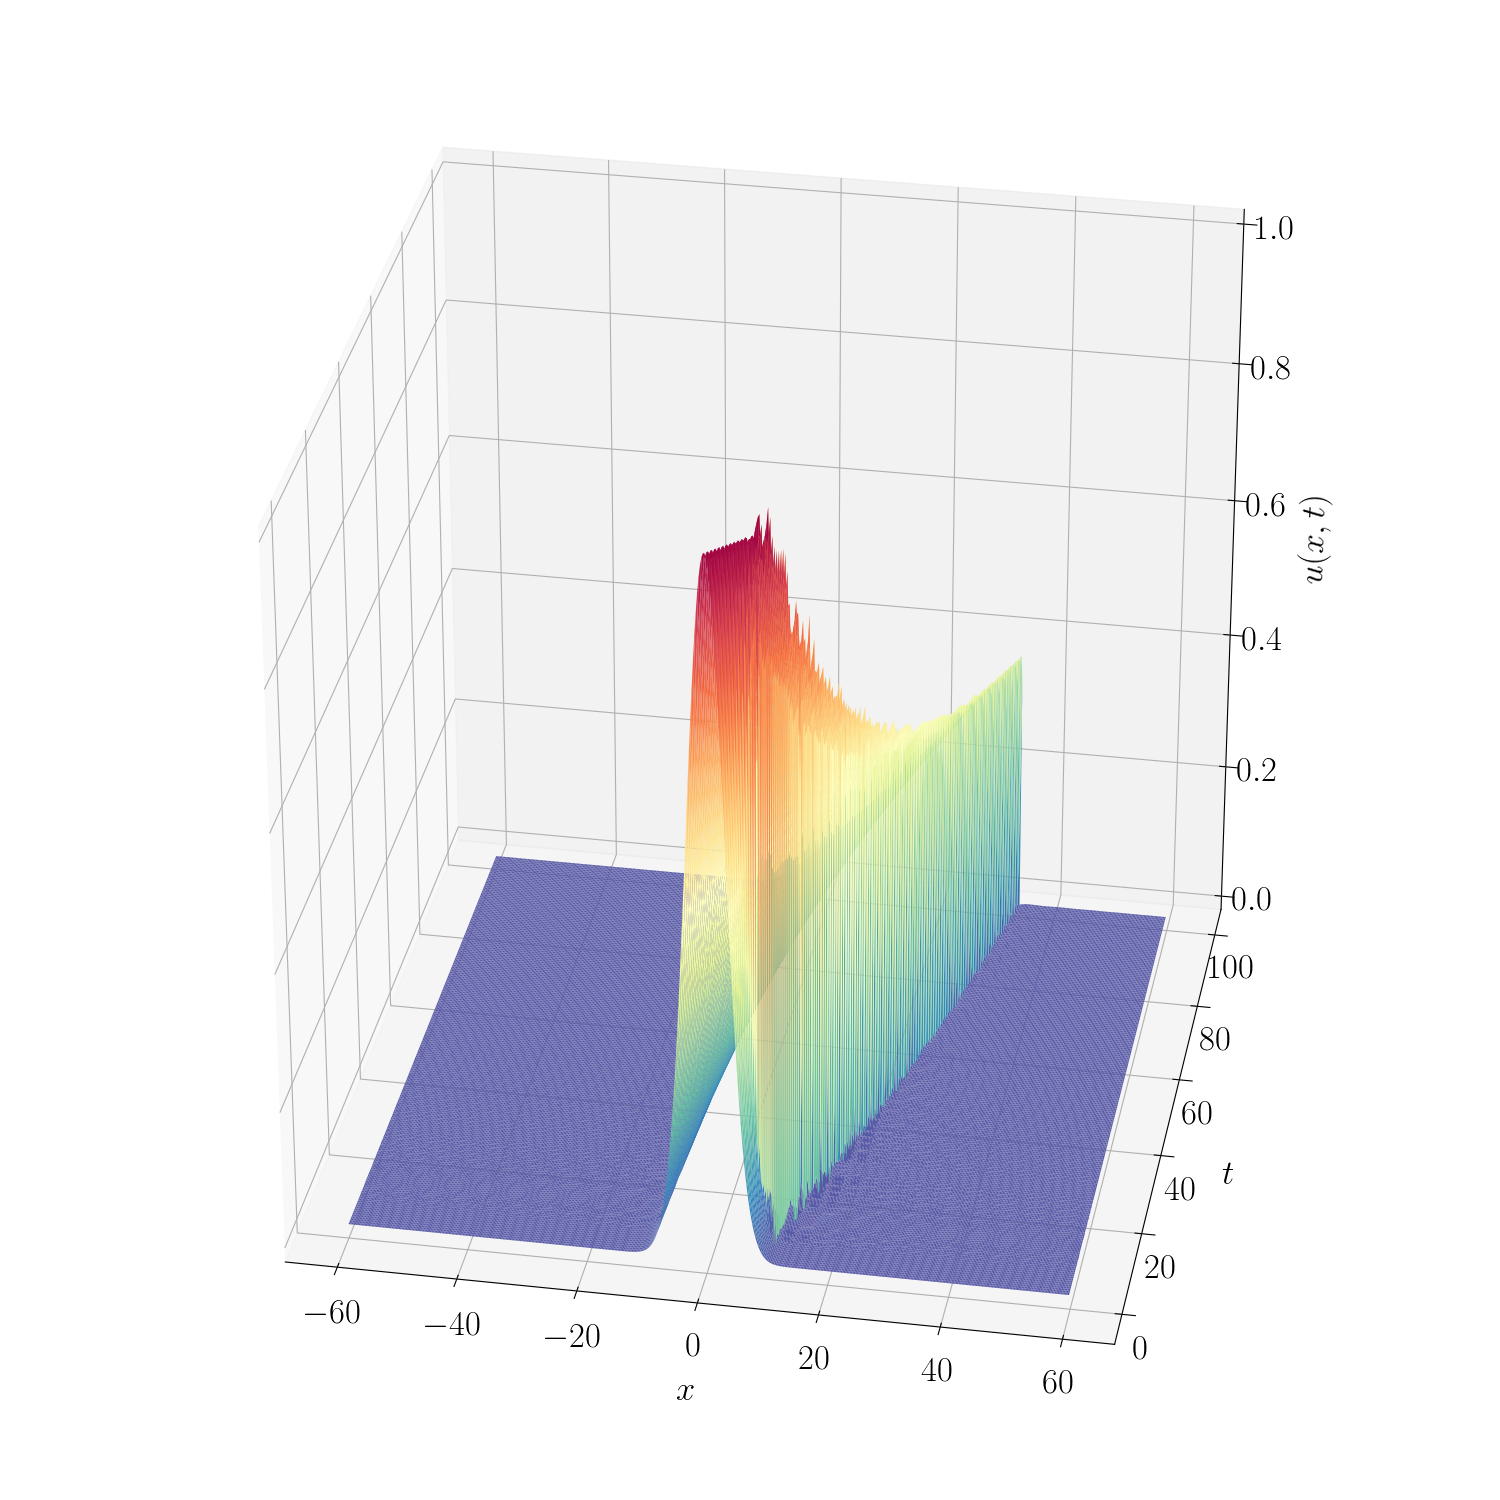
\includegraphics[height=5cm,width=4cm]{files/figures/viscid/galerkin/Numerical_Solution_alpha=0005.png}
        \qquad
        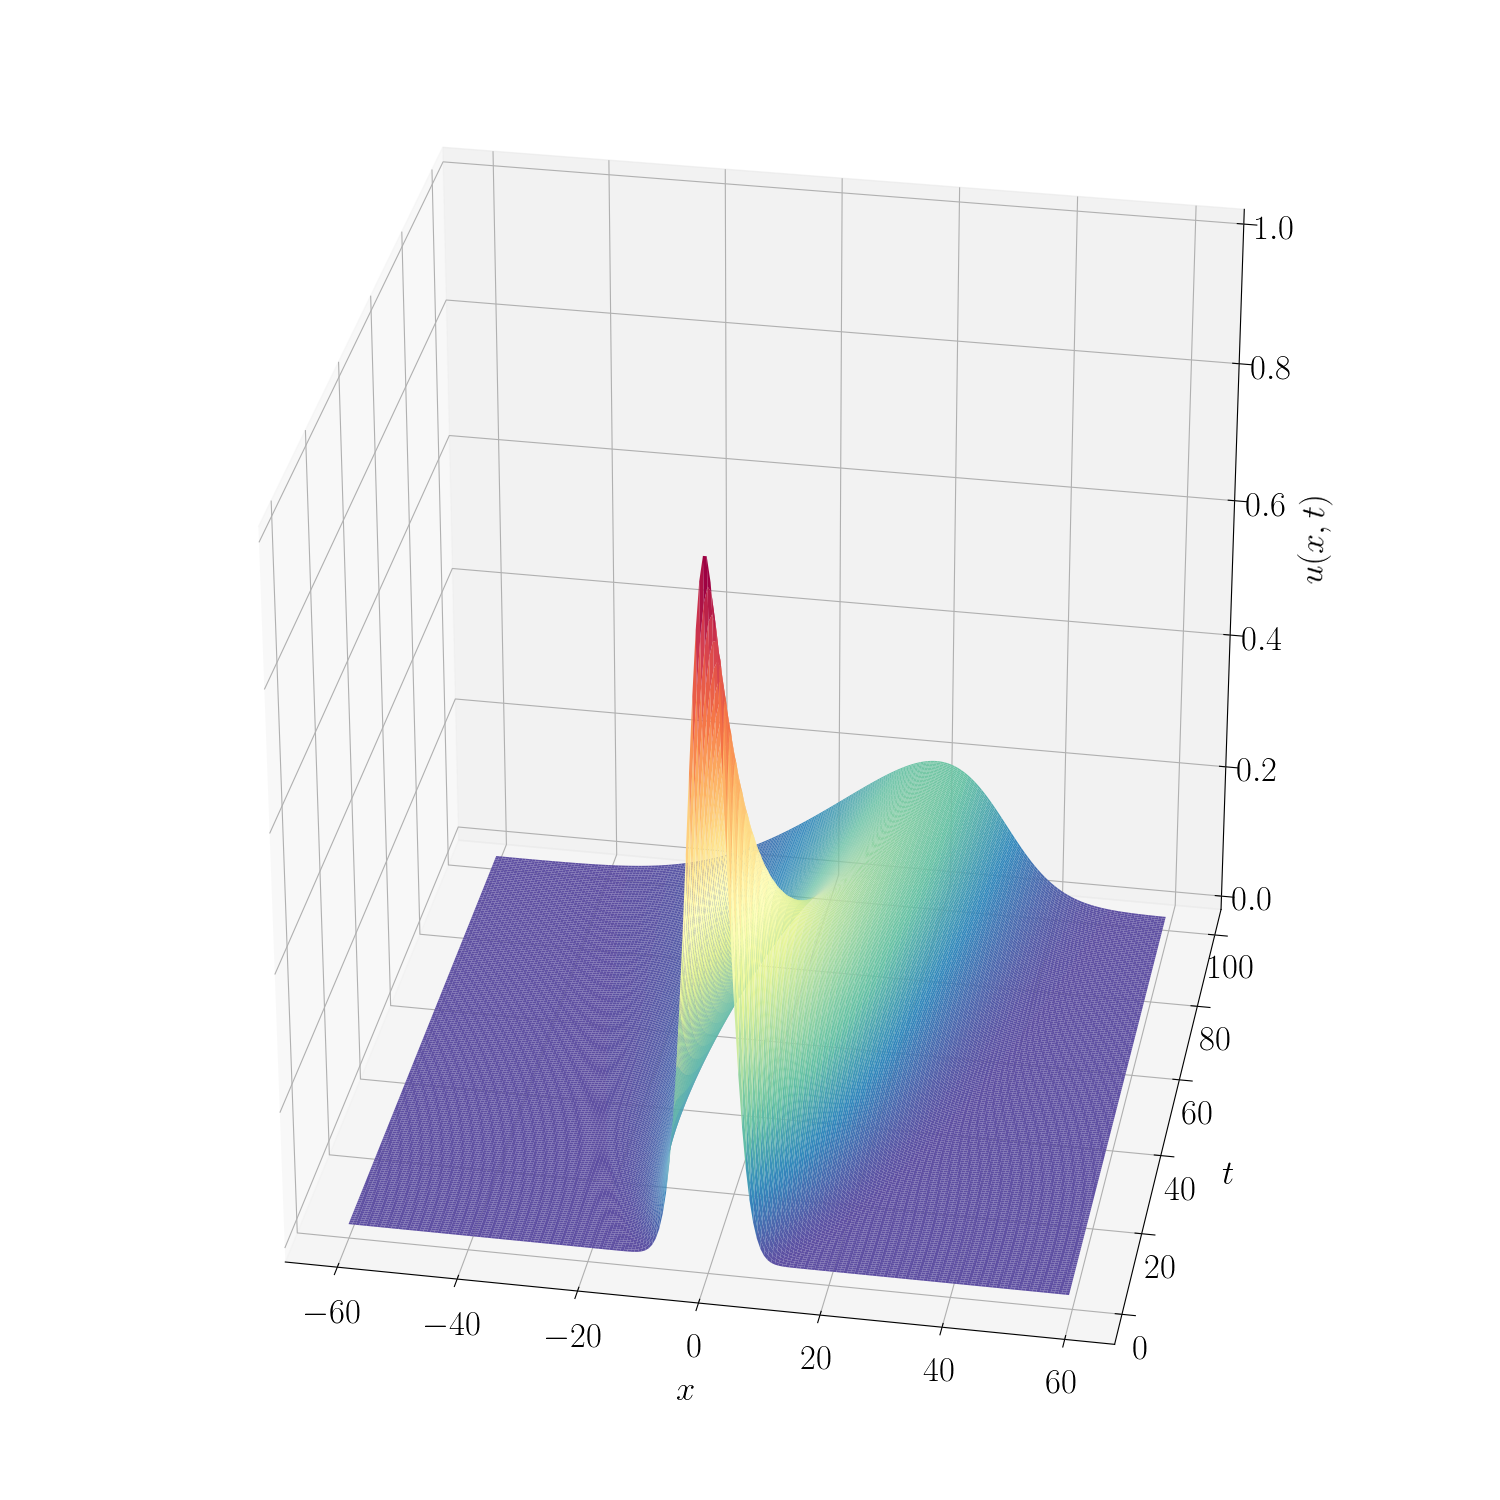
\includegraphics[height=5cm,width=4cm]{files/figures/viscid/galerkin/Numerical_Solution_alpha=1.png}
        \caption{ $\alpha = 0.005$; $N=2048$; $\Delta t = 1.0 \times 10^{-5}$ (b) $\alpha = 1.0$; $N=2048$; $\Delta t = 1.0 \times 10^{-5}$.}
    \end{figure}
\end{frame}

\begin{frame}{Simulaciones: Fourier-Galerkin \hspace{2cm} \hyperlink{Navegador}{\beamergotobutton{Navegador}}}
    \begin{figure}
    	\centering
    	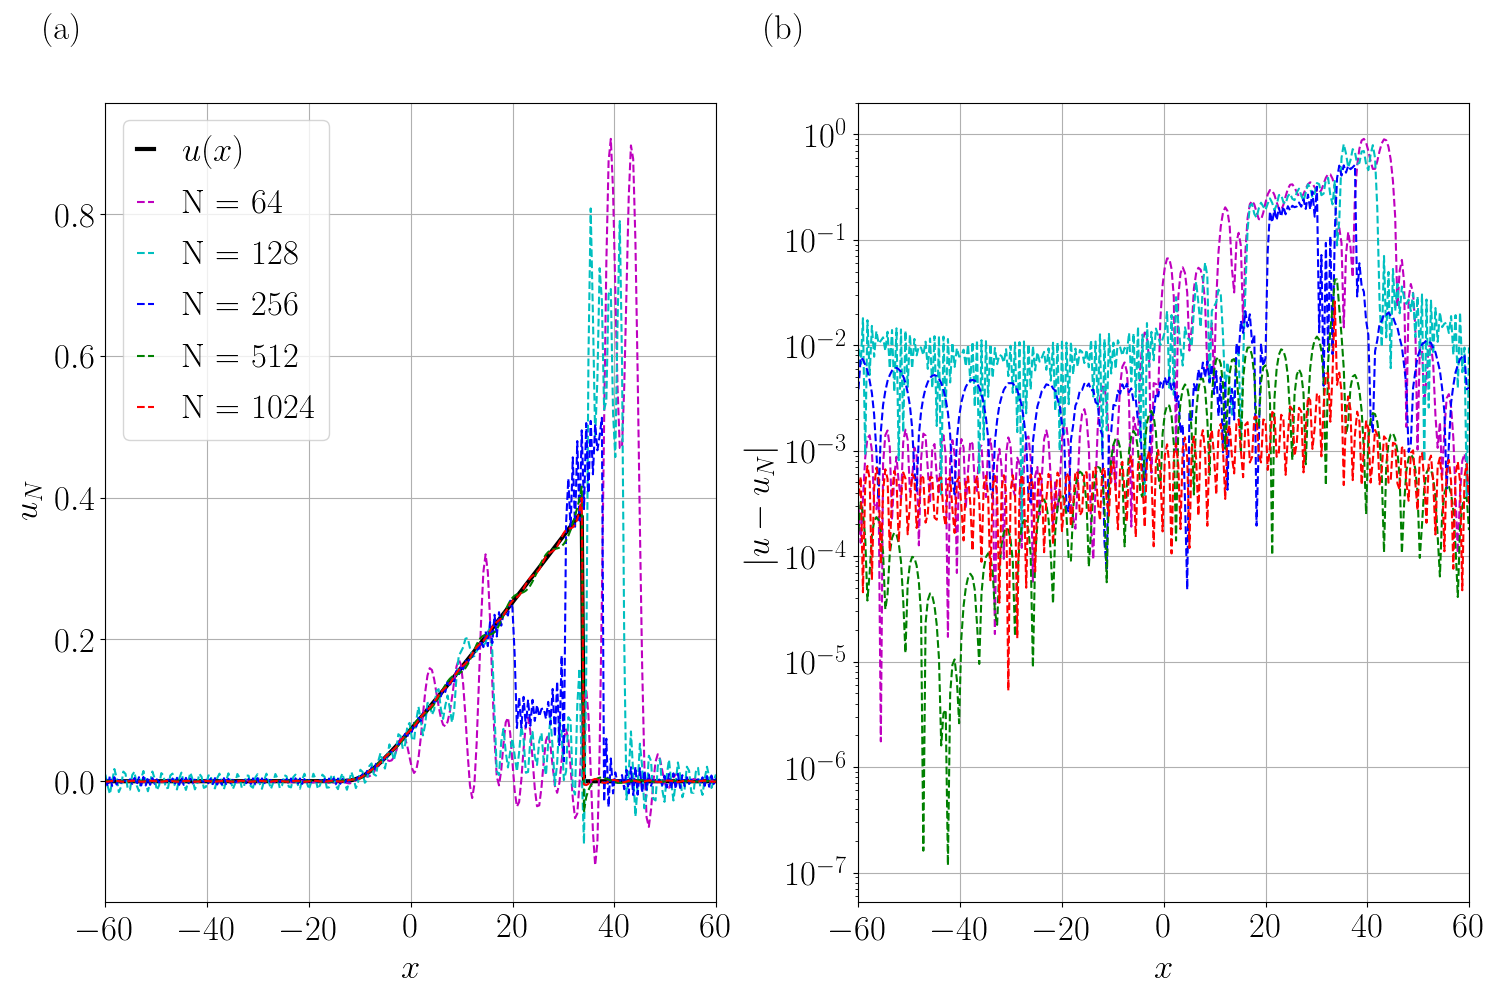
\includegraphics[height=5cm,width=4cm]{files/figures/viscid/galerkin/Numerical_Solution_alpha=0005_T=100.png}
        \qquad
    	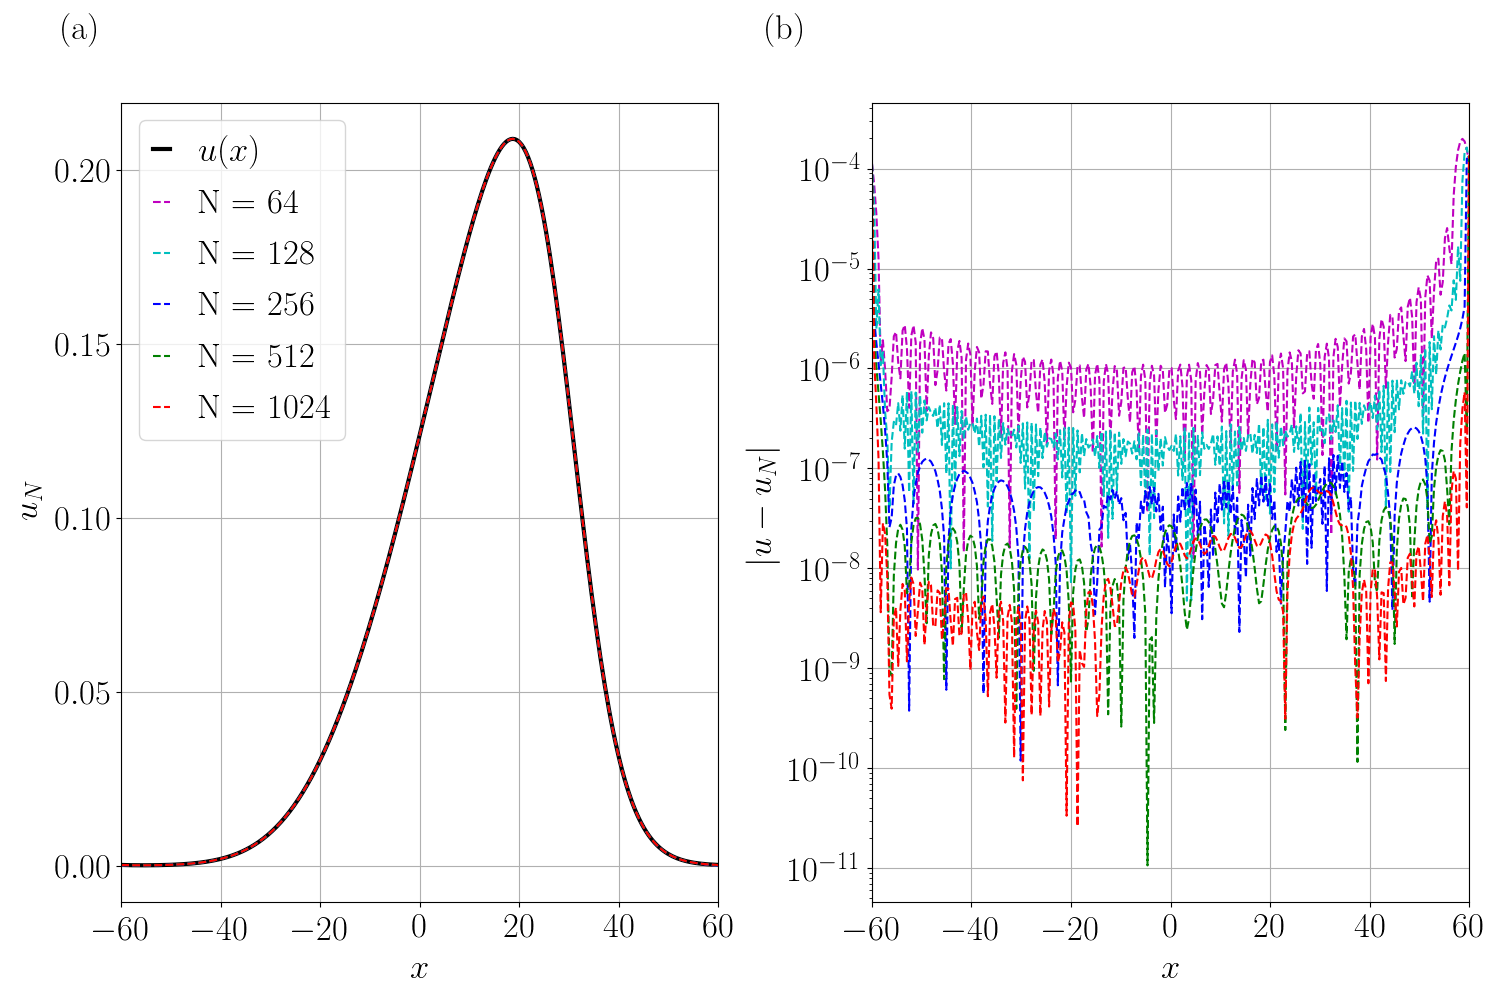
\includegraphics[height=5cm,width=4cm]{files/figures/viscid/galerkin/Numerical_Solution_alpha=1_T=100.png}
        \caption{(a) $t = 100$; $\alpha = 0.005$; $\Delta t = 1.0 \times 10^{-5}$ (b) $t = 100$, $\alpha = 1.0$, $\Delta t = 1.0 \times 10^{-5}$.}
    \end{figure}
\end{frame}

\label{Tablas-Galerkin}
\begin{frame}{Simulaciones: Fourier-Galerkin \hspace{2cm} \hyperlink{Navegador}{\beamergotobutton{Navegador}}}
    \begin{table}
        \centering
        \begin{tabular}{lccc}
        	\toprule
        	\multicolumn{1}{c}{} &\multicolumn{3}{c}{\textbf{Error}} \\
        	N &$\Delta t=1\times 10^{-3}$ &$\Delta t=1\times 10^{-4}$ &$\Delta t=1\times 10^{-5}$ \\
        	\midrule
        	16&0.72504 &0.72504 &0.72504 \\
        	\midrule
        	32& 6.88052 $\times 10 ^{-2}$& 6.87838 $\times 10 ^{-2}$& 6.87816 $\times 10 ^{-2}$ \\
        	\midrule
        	64& 8.85367 $\times 10 ^{-4}$& 8.80521 $\times 10 ^{-4}$& 8.80410 $\times 10 ^{-4}$ \\
        	\midrule
        	128& 9.41793 $\times 10 ^{-5}$& 9.41148 $\times 10 ^{-6}$& 9.41827 $\times 10 ^{-7}$ \\
        	\midrule
        	256& 9.41793 $\times 10 ^{-5}$& 9.41109 $\times 10 ^{-6}$& 9.36411 $\times 10 ^{-7}$ \\
        	\midrule
        	512& 9.41793 $\times 10 ^{-5}$& 9.41109 $\times 10 ^{-6}$& 9.36411 $\times 10 ^{-7}$ \\
        	\bottomrule
        \end{tabular}
        \caption{Error $L_2$}
    \end{table}
\end{frame}

\begin{frame}{Simulaciones: Fourier-Galerkin \hspace{2cm} \hyperlink{Navegador}{\beamergotobutton{Navegador}}}
    \begin{table}
	\centering
	\begin{tabular}{lccc}
		\toprule
		\multicolumn{1}{c}{}& \multicolumn{3}{c}{\textbf{Error}} \\
		$N$& $\Delta t=1\times 10^{-3}$& $\Delta t=1\times 10^{-4}$& $\Delta t=1\times 10^{-5}$ \\
		\midrule
		16& 9.91901& 9.91597& 9.91567 \\
		\midrule
		32& 2.70558& 2.70347& 2.70326 \\
		\midrule
		64& 2.45988& 2.45543& 2.45497 \\
		\midrule
		128& 2.06992& 2.05918& 2.05795 \\
		\midrule
		256& 1.19385& 1.17602& 1.17412 \\
		\midrule
		512& 0.265843& 0.262164& 0.261805 \\
		\midrule
		1024& 0.133743& 0.131882& 0.131699 \\
		\midrule
		2048& 4.70602 $\times 10^{-2}$& 4.57371 $\times 10^{-2}$& 4.56090 $\times 10^{-2}$ \\
		\midrule
		4096& 7.26917 $\times 10^{-3}$& 6.64157 $\times 10^{-3}$& 6.60753 $\times 10^{-3}$ \\
		\bottomrule
	\end{tabular}
	\caption{Error $L_2$}
\end{table}
\end{frame}
%========================
\label{Figuras-Cero-Viscosidad}
\begin{frame}{Simulaciones: Fourier-Galerkin \hspace{2cm} \hyperlink{Navegador}{\beamergotobutton{Navegador}}}
    \begin{figure}
        \centering
        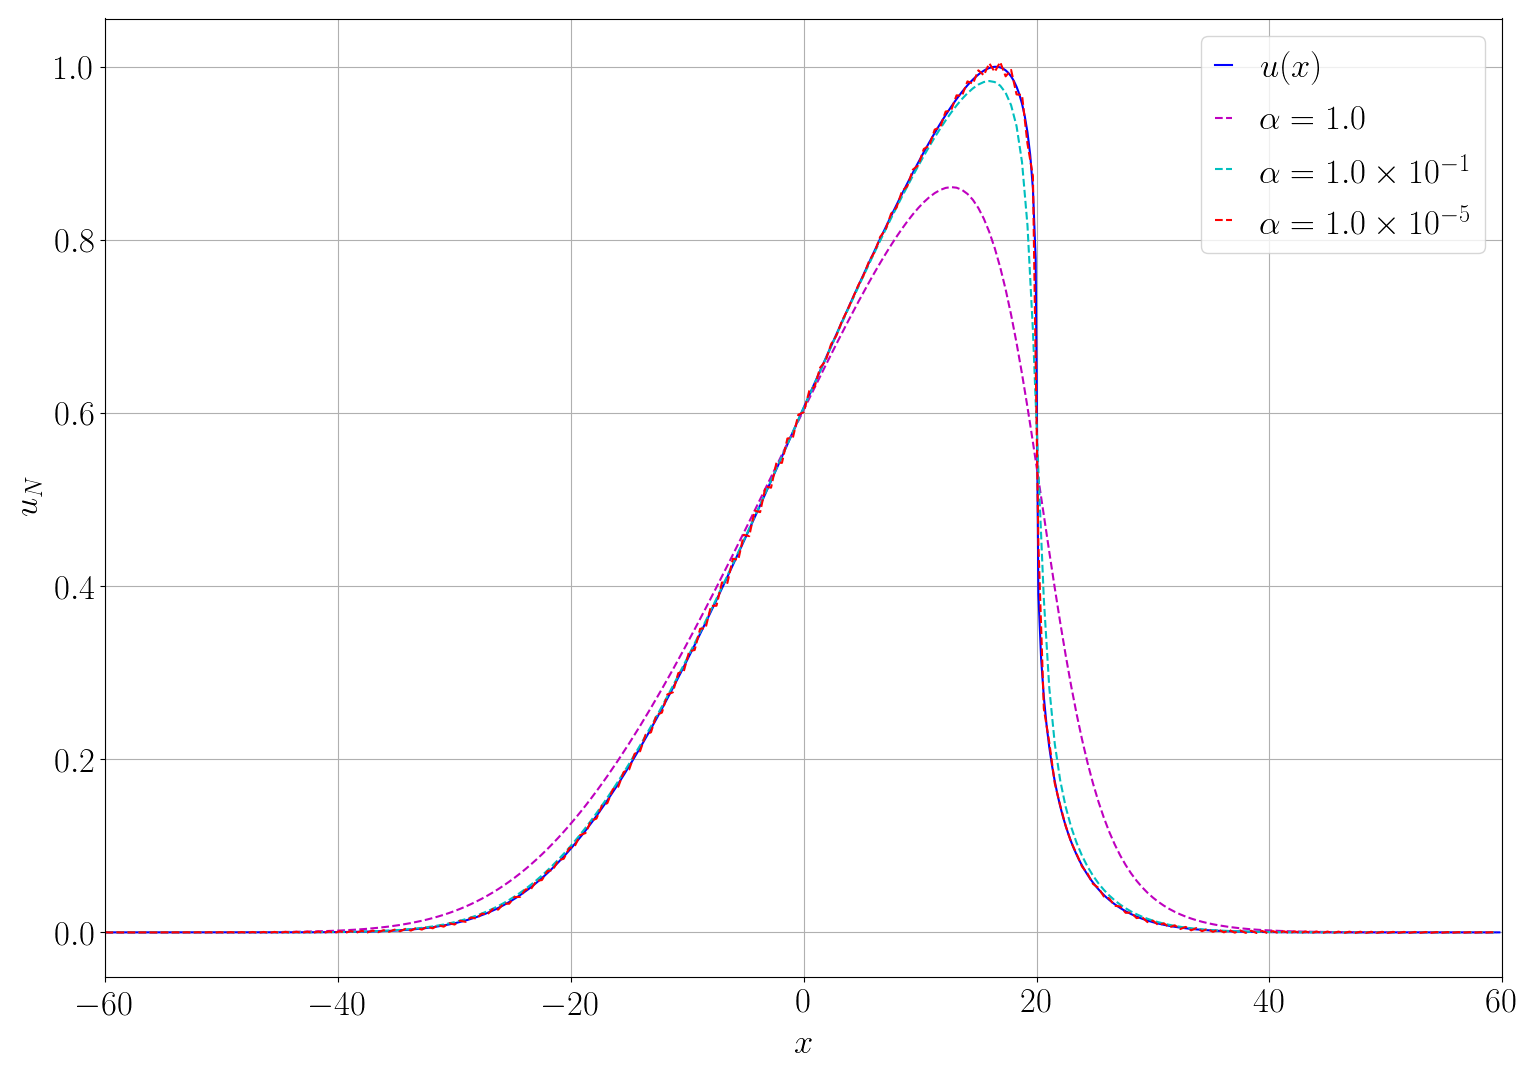
\includegraphics[height=5cm,width=4cm]{files/figures/inviscid/varios_alphas.png}
        \qquad
        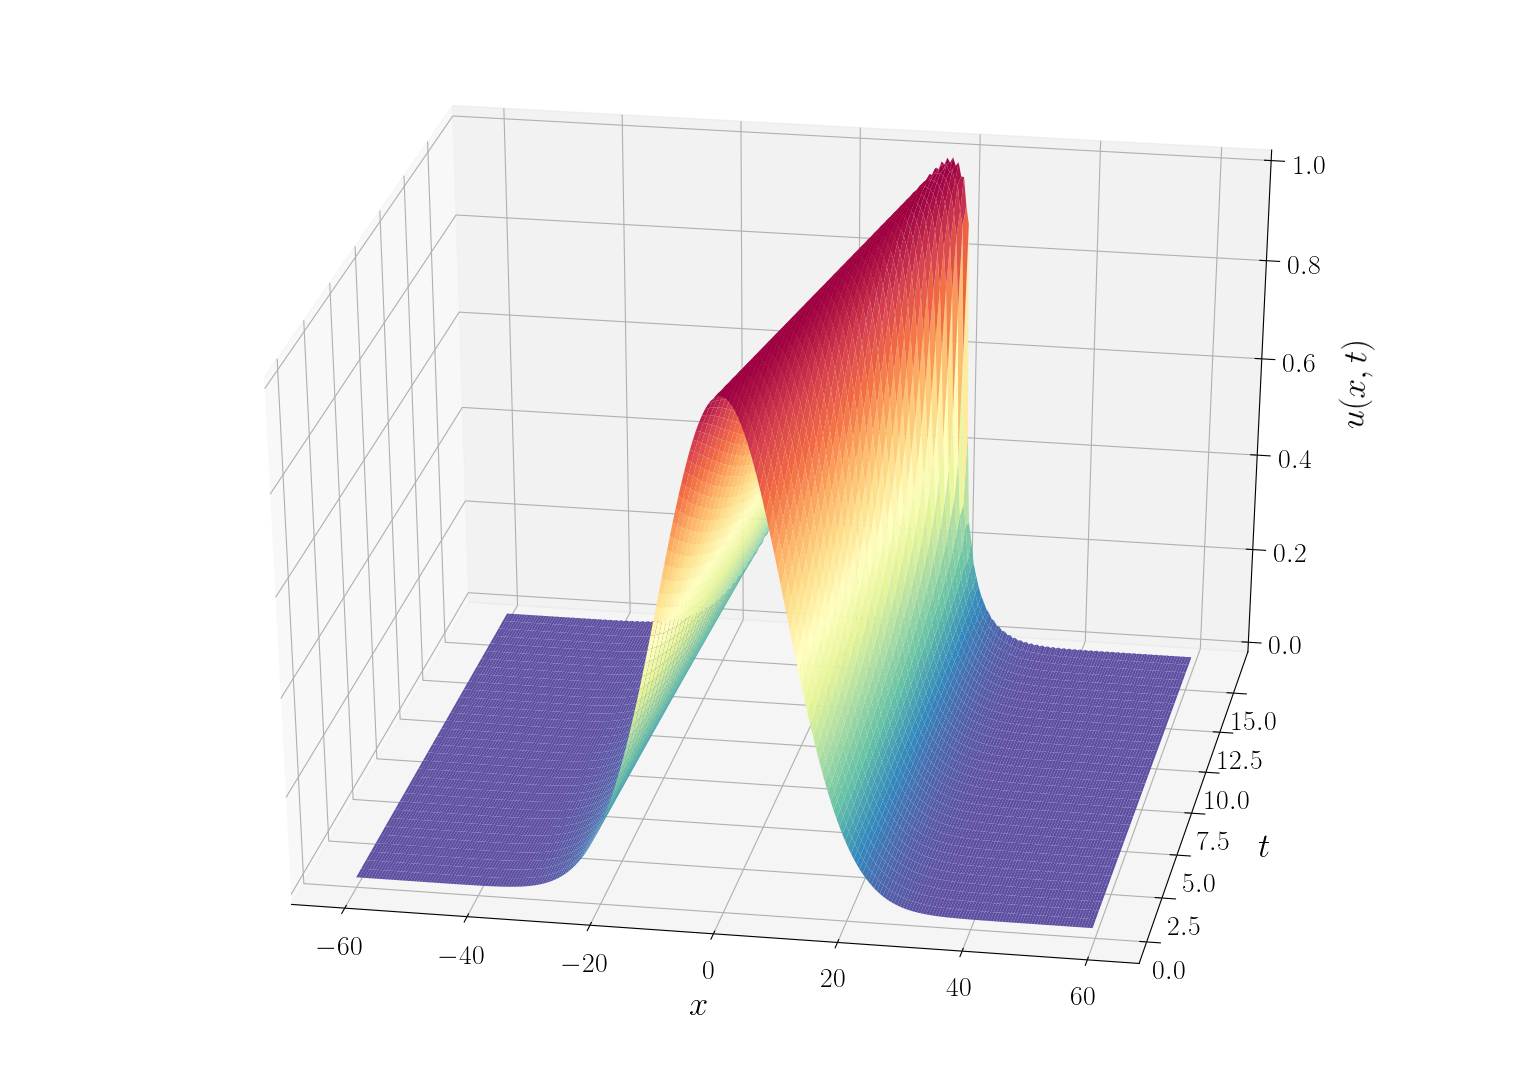
\includegraphics[height=5cm,width=4cm]{files/figures/inviscid/small_alpha.png}
        \caption{(a) $t = T_c, N=256, \Delta t = 1., \times 10^{-3}.$ (b) $\alpha = 1.0, \times 10^{-5}, N=256, \Delta t = 1.0, \times 10^{-3}.$}
    \end{figure}    
\end{frame}

\begin{frame}{Simulaciones: Fourier-Galerkin \hspace{2cm} \hyperlink{Navegador}{\beamergotobutton{Navegador}}}
    \begin{figure}
        \centering
        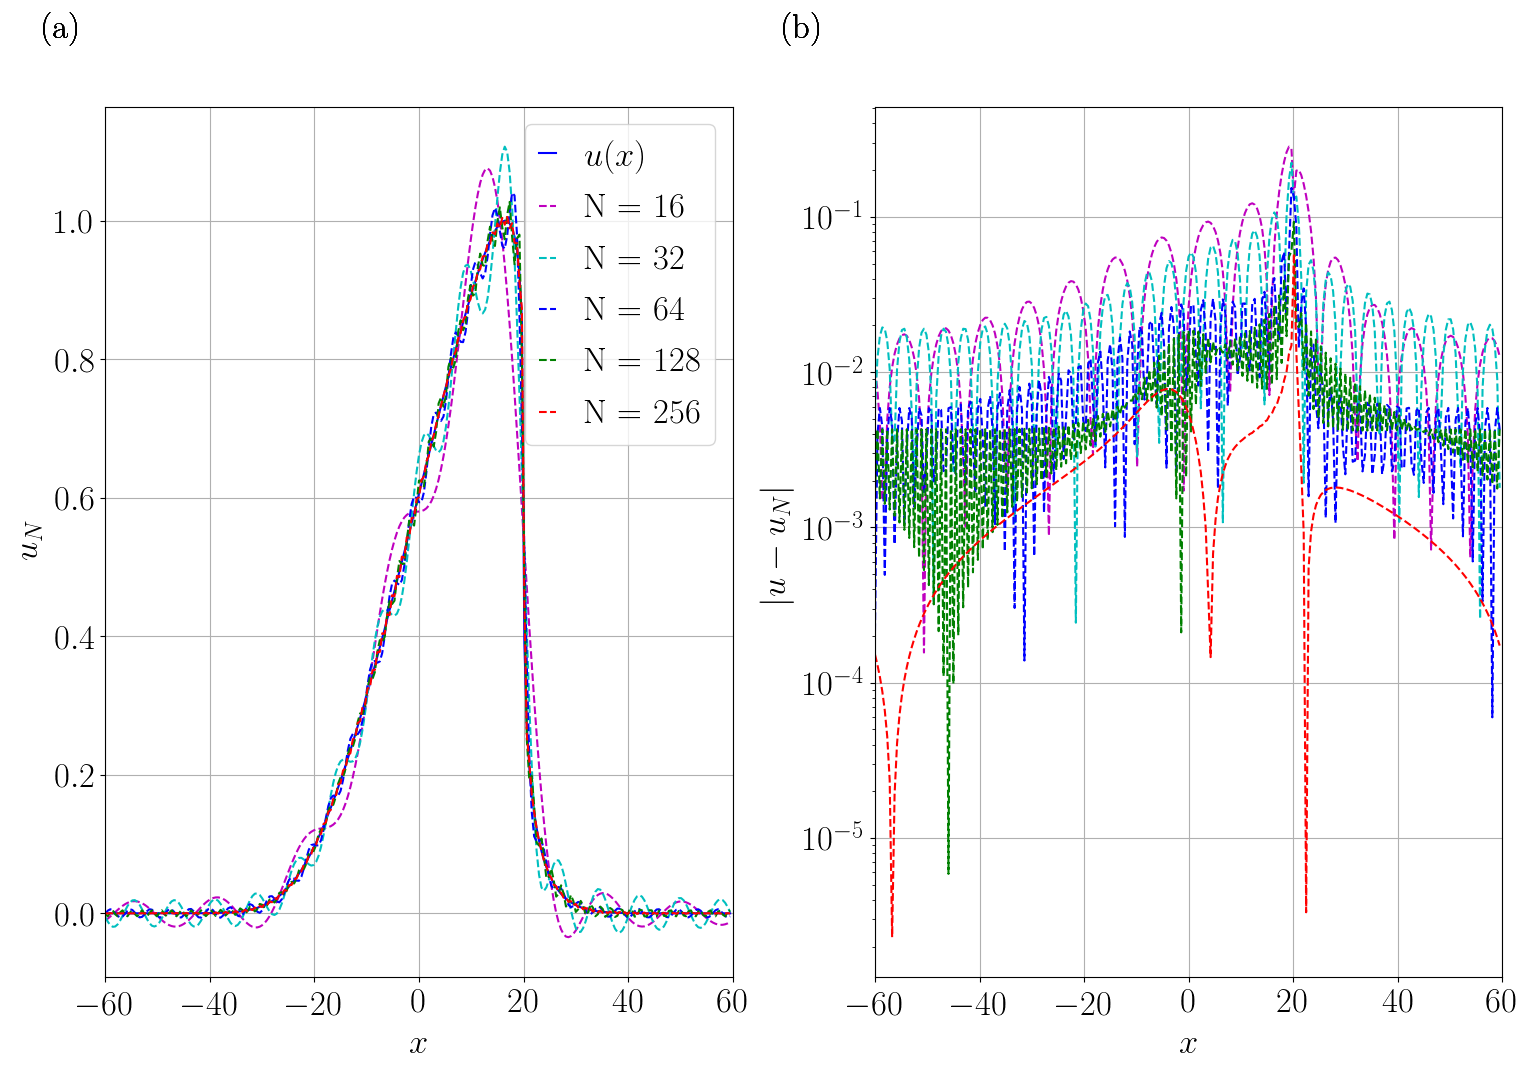
\includegraphics[height=6cm,width=8cm]{files/figures/inviscid/small_alpha_T.png}
        \caption{$t = T_c$; $\alpha = 1.0 \times 10^{-5}$; $\Delta t = 1.0 \times 10^{-3}$}
    \end{figure}
\end{frame}

\begin{frame}{Simulaciones: Fourier-Galerkin \hspace{2cm} \hyperlink{Navegador}{\beamergotobutton{Navegador}}}    
	\begin{table}
		\centering
		\begin{tabular}{lccc}
			\toprule
			\multicolumn{1}{c}{}& \multicolumn{3}{c}{\textbf{Distance}} \\
			$N$& $\Delta t=1\times 10^{-2}$& $\Delta t=1\times 10^{-3}$& $\Delta t=1\times 10^{-4}$ \\
			\midrule
			16& 0.285531& 0.285732& 0.285752 \\
			\midrule
			32& 0.222737& 0.223260& 0.223312 \\
			\midrule
			64& 0.160385& 0.162782& 0.163025 \\
			\midrule
			128& 0.129297& 0.133322& 0.133733 \\
			\midrule
			256& 0.083291& 0.091449& 0.092320 \\
			\bottomrule
		\end{tabular}
		\caption{Error $L_2$}
	\end{table}
\end{frame}
%==========================
\label{Figuras-Colocacion}
\begin{frame}{Simulaciones: Fourier-Colocacion \hspace{2cm} \hyperlink{Navegador}{\beamergotobutton{Navegador}}}
    \begin{figure}
	    \centering
    	\includegraphics[height=6cm,width=10cm]{files/figures/viscid/collocation/alphas_Error_N.png}
    	\caption{$\alpha = 1.0$; $N=2048$; $\Delta t = 1.0 \times 10^{-5}$.}
	\end{figure}
\end{frame}

\begin{frame}{Simulaciones: Fourier-Colocacion \hspace{2cm} \hyperlink{Navegador}{\beamergotobutton{Navegador}}}
	\begin{figure}
	    \centering
    	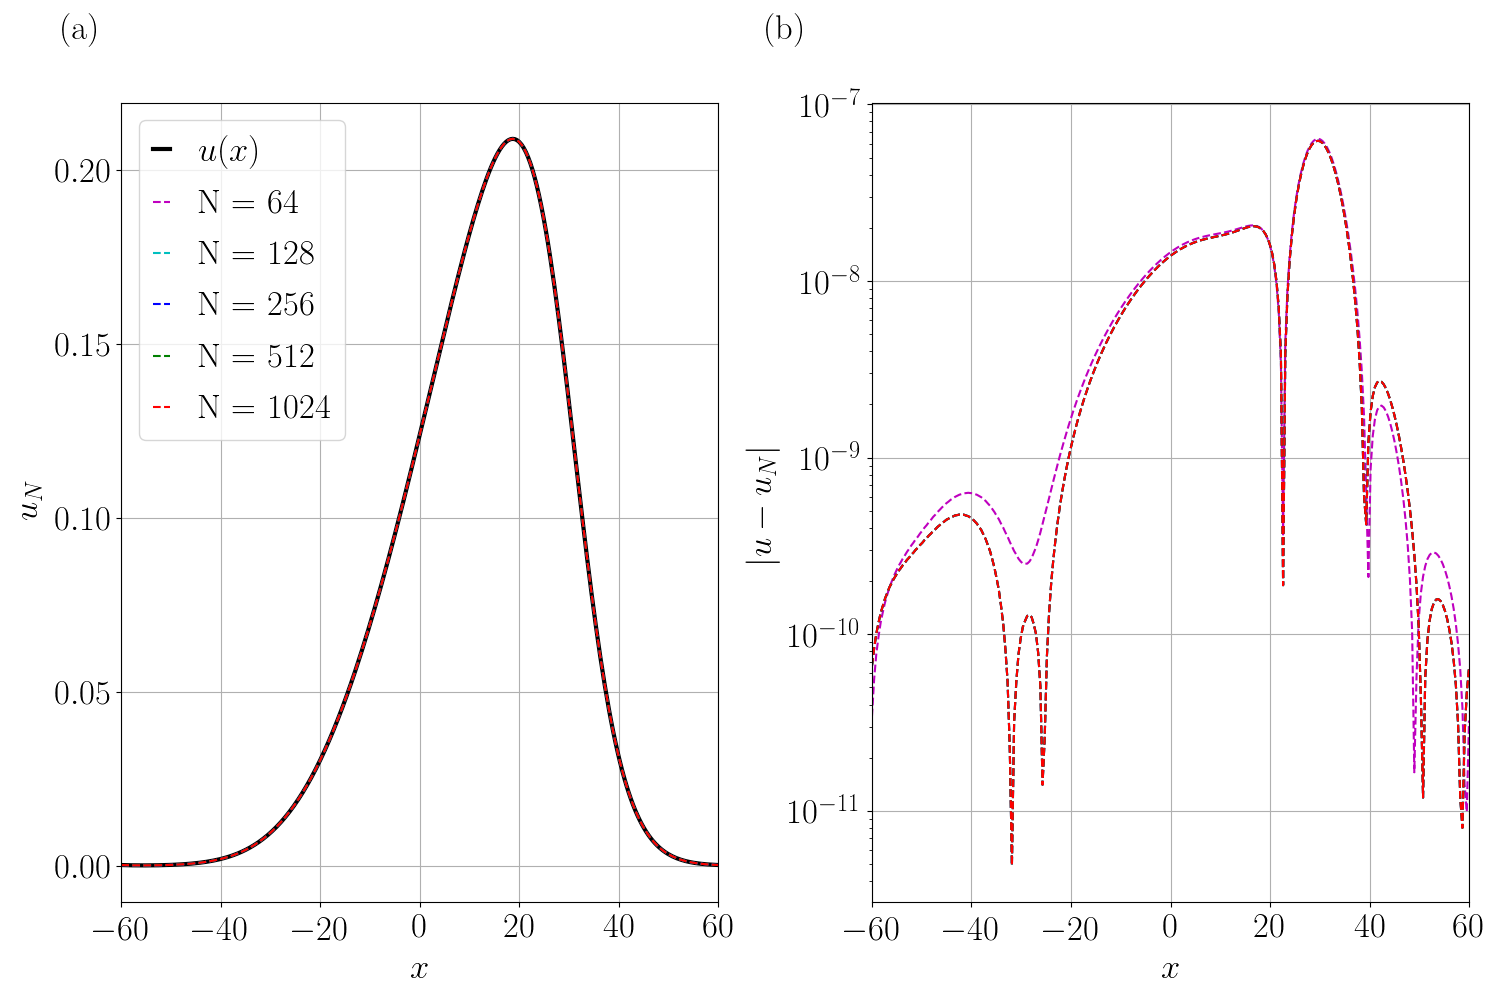
\includegraphics[height=5cm,width=4cm]{files/figures/viscid/collocation/Numerical_Solution_alpha=1_T=100.png}
        \qquad
	    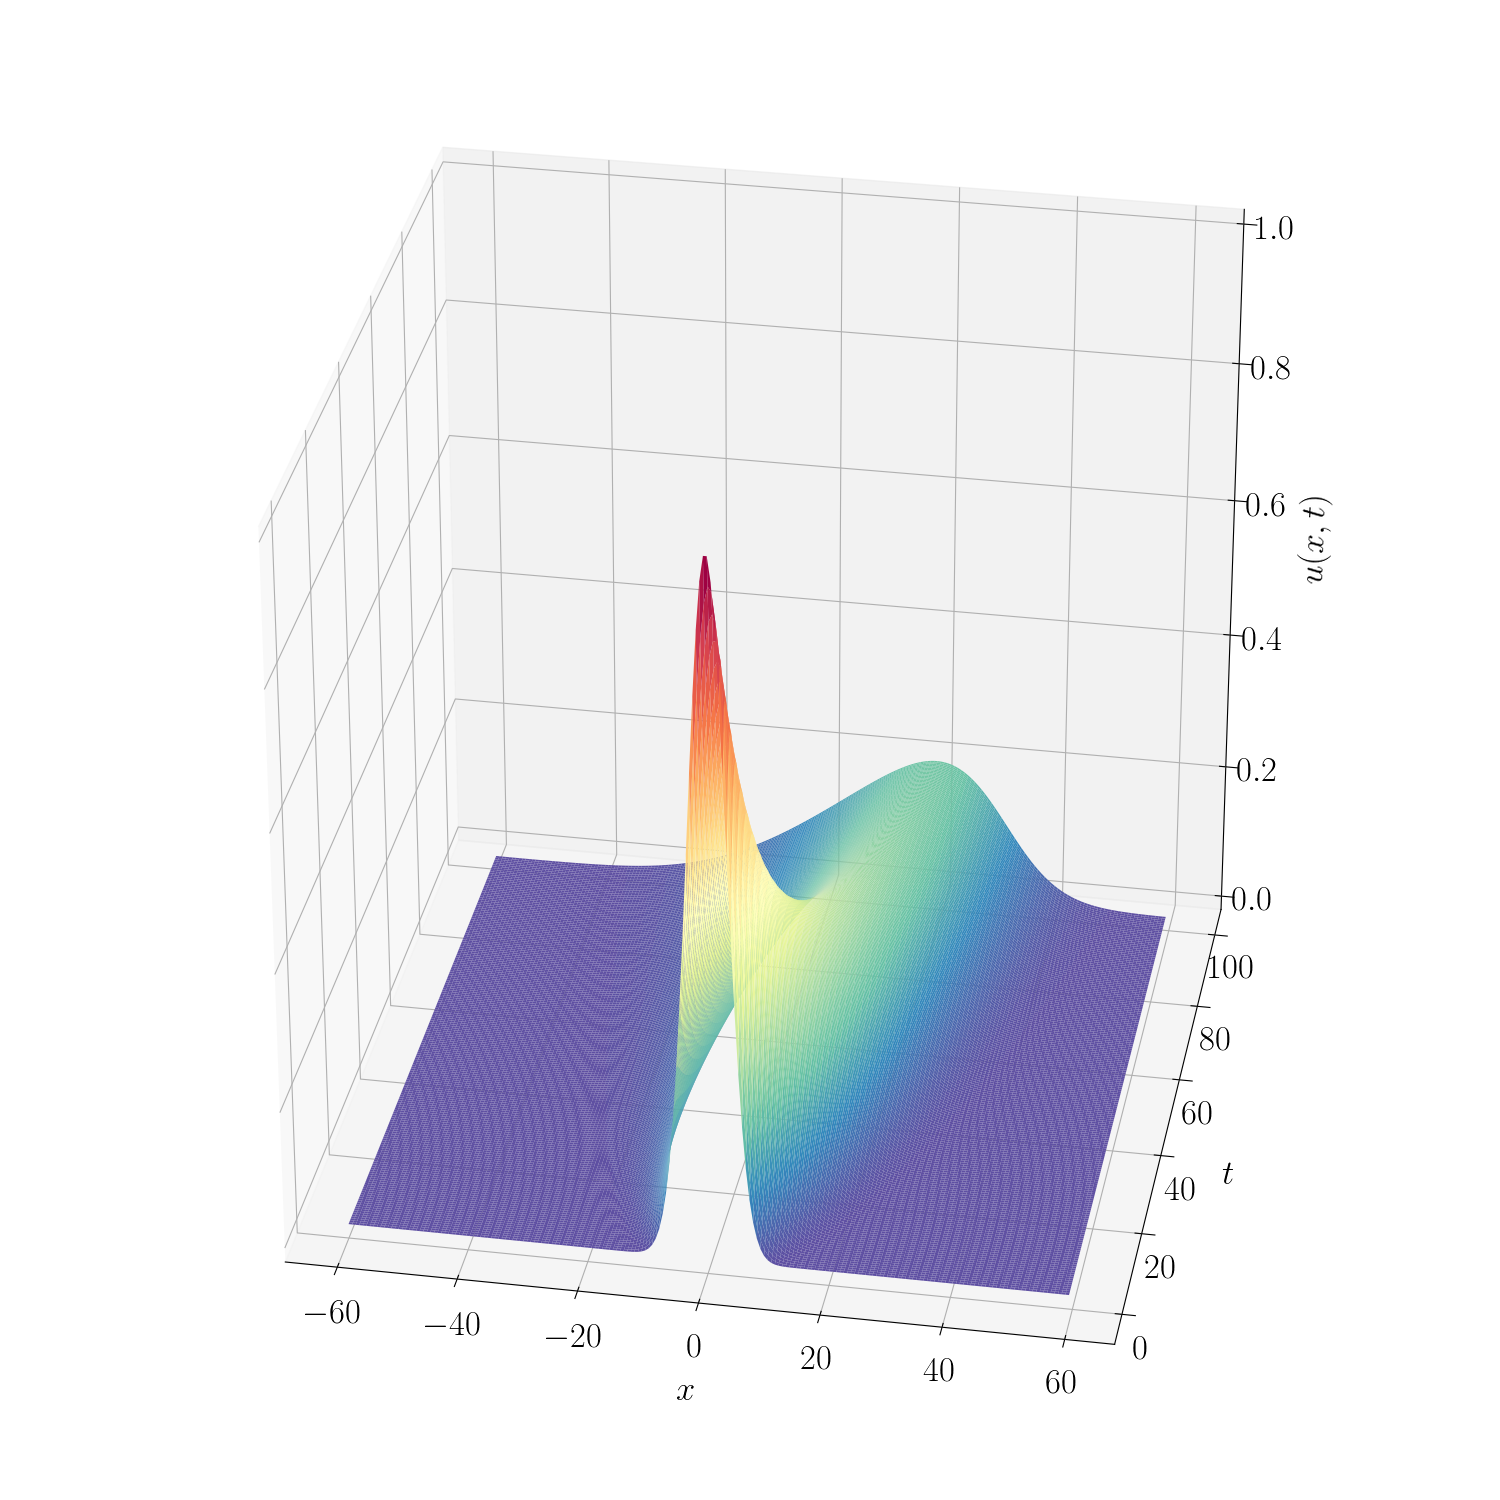
\includegraphics[height=5cm,width=4cm]{files/figures/viscid/collocation/Numerical_Solution_alpha=1.png}
    	\caption{(a) $t = 100$, $\alpha = 1.0$, $\Delta t = 1.0 \times 10^{-5}$. (b) $\alpha = 1.0$; $N=2048$; $\Delta t = 1.0 \times 10^{-5}$.}
	\end{figure}
\end{frame}

\begin{frame}{Simulaciones: Fourier-Colocacion \hspace{2cm} \hyperlink{Navegador}{\beamergotobutton{Navegador}}}
		\begin{figure}
	    \centering
	    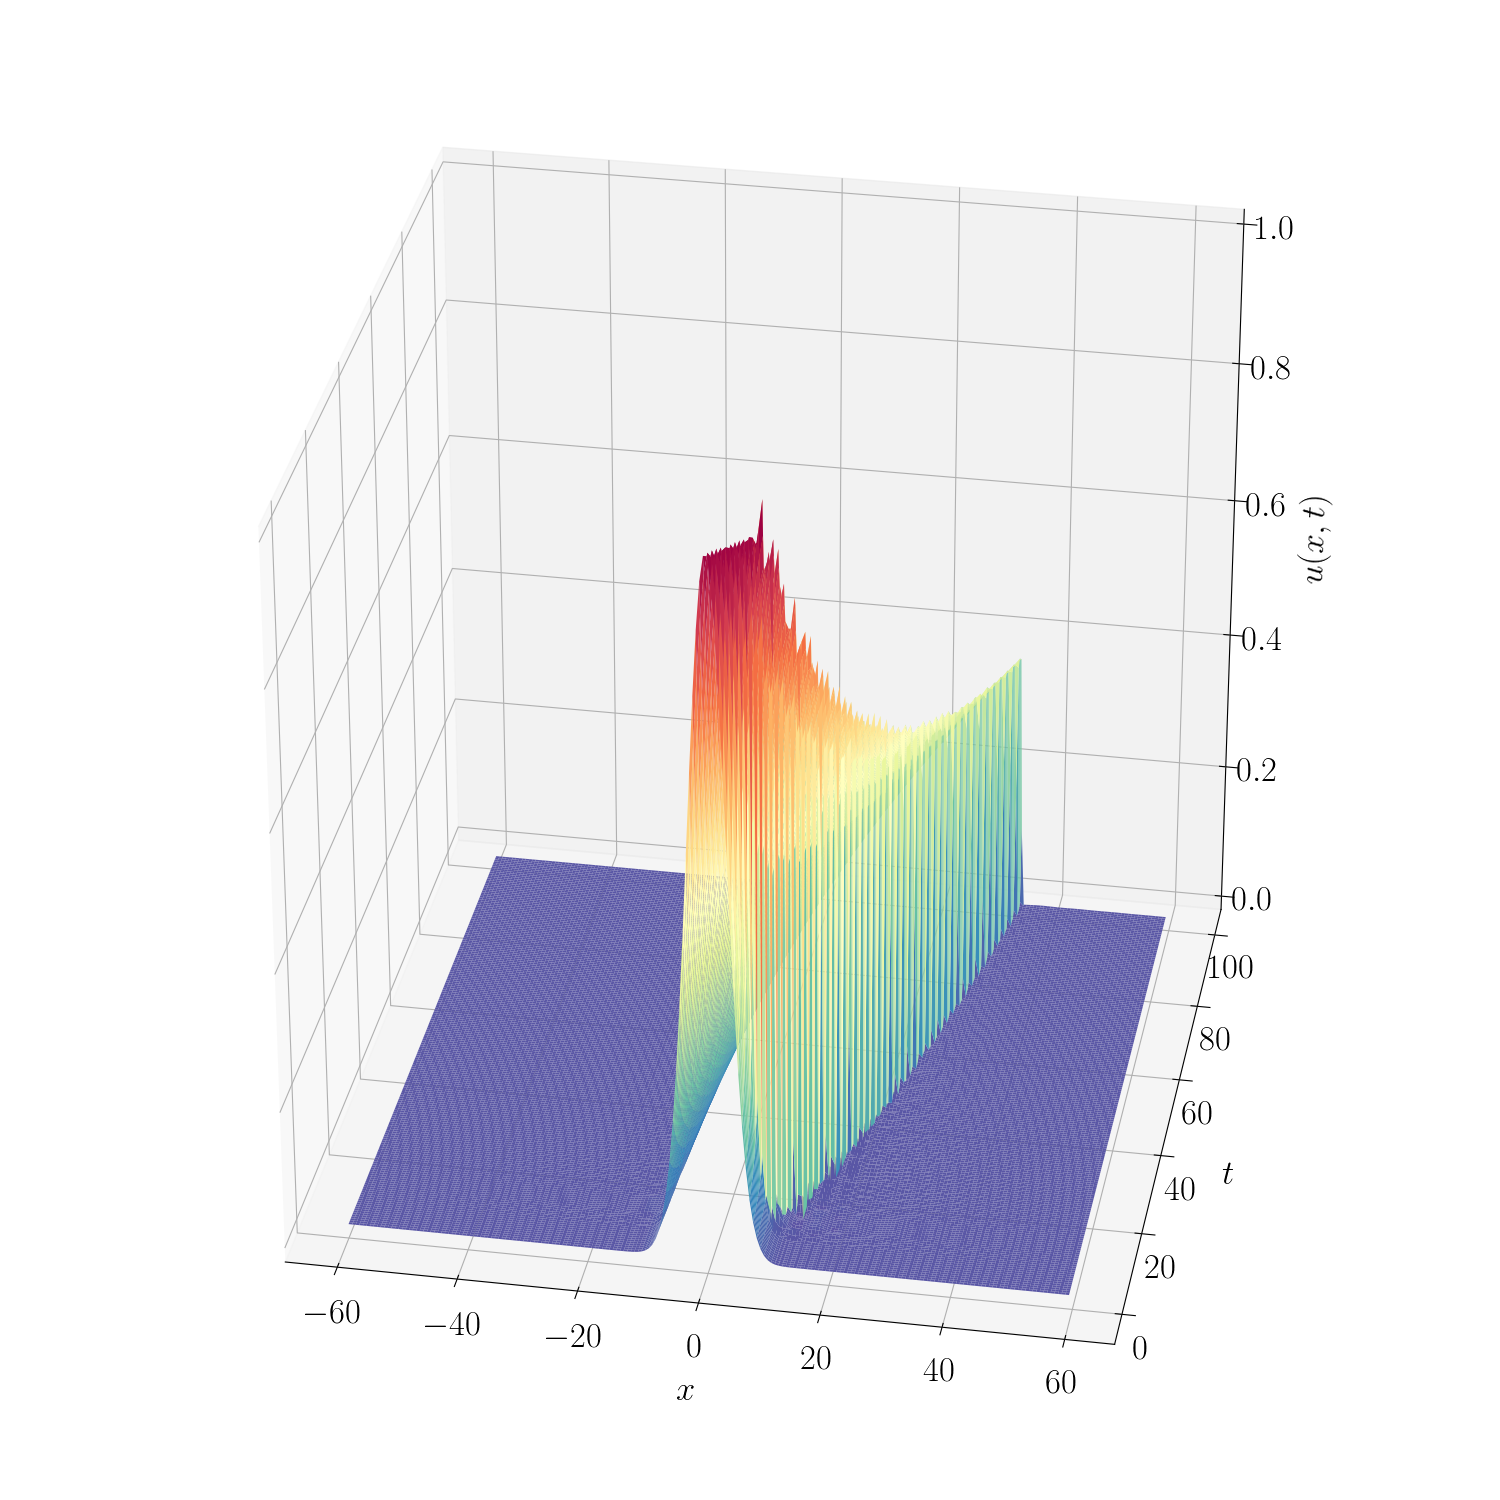
\includegraphics[height=5cm,width=4cm]{files/figures/viscid/collocation/Numerical_Solution_alpha=0005.png}
	    \qquad
	    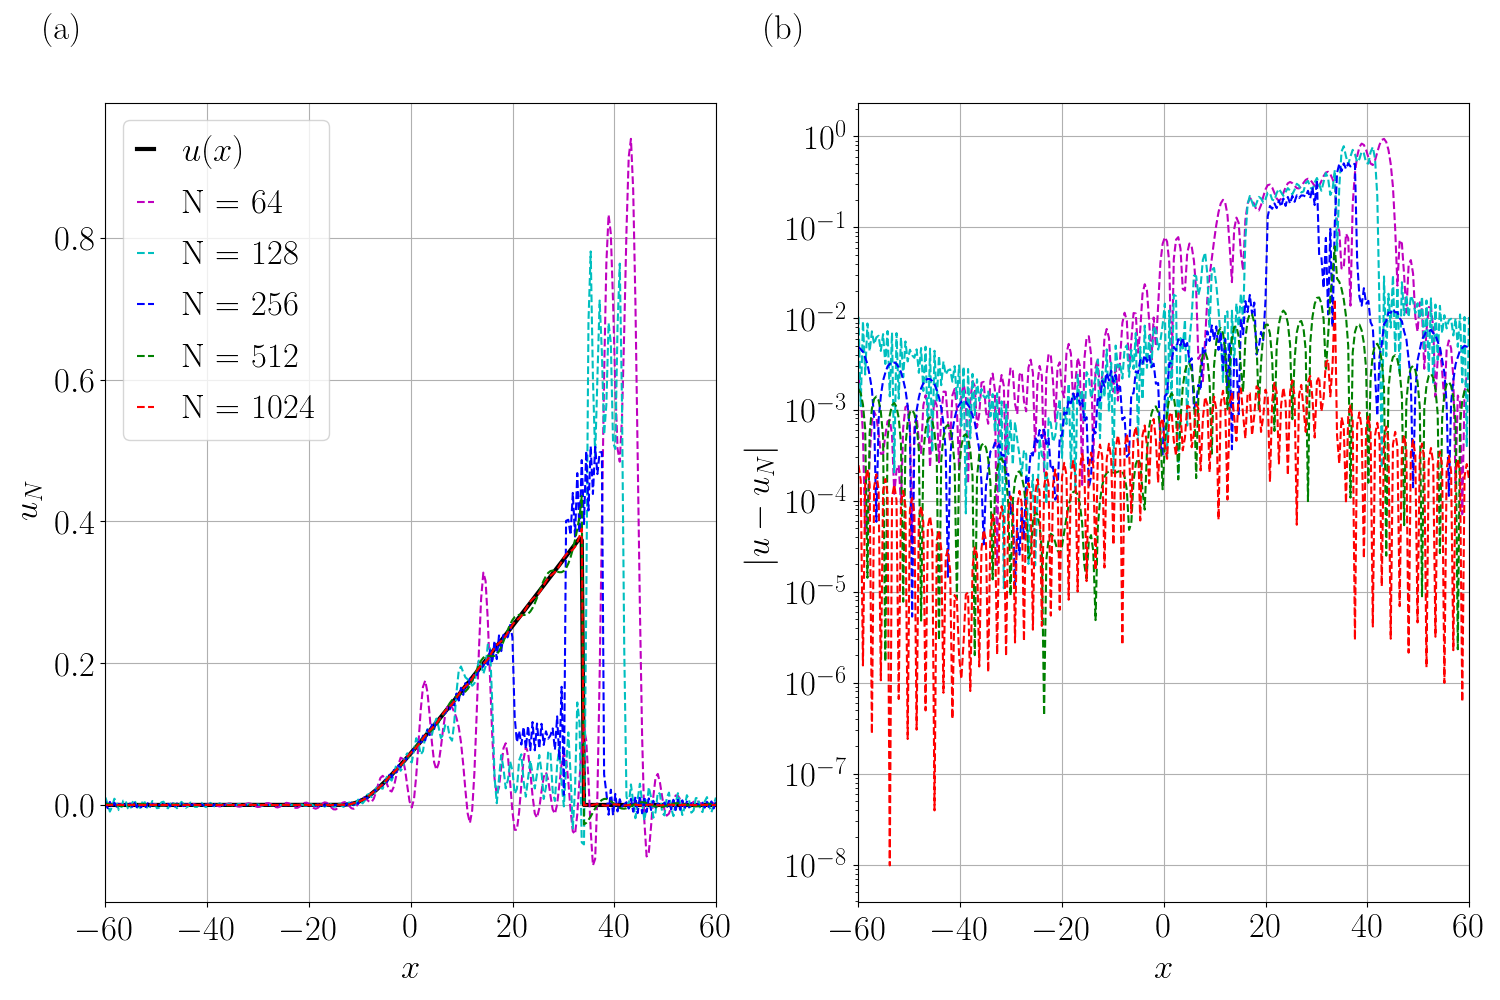
\includegraphics[height=5cm,width=4cm]{files/figures/viscid/collocation/Numerical_Solution_alpha=0005_T=100.png}
    	\caption{(a) $\alpha = 0.005$; $N=2048$; $\Delta t = 1.0 \times 10^{-5}$ (b) $t = 100$, $\alpha = 0.005$, $\Delta t = 1.0 \times 10^{-5}$.}
	\end{figure}
\end{frame}

\label{Tablas-Colocacion}
\begin{frame}{Simulaciones: Fourier-Colocacion \hspace{2cm} \hyperlink{Navegador}{\beamergotobutton{Navegador}}}
	\begin{table}
    \centering
	\begin{tabular}{lccc}
		\toprule
		\multicolumn{1}{c}{}& \multicolumn{3}{c}{\textbf{Error}} \\
		$N$& $\Delta t=1\times 10^{-3}$& $\Delta t=1\times 10^{-4}$& $\Delta t=1\times 10^{-5}$ \\
		\midrule
		16& 0.721112& 0.721112& 0.721112 \\
		\midrule
		32& 4.73004 $\times 10^{-2}$& 4.73015 $\times 10^{-2}$ \\
		\midrule
		64& 7.35344 $\times 10^{-4}$& 7.27561 $\times 10^{-4}$& 7.27283 $\times 10^{-4}$ \\
		\midrule
		128& 1.75152 $\times 10^{-5}$& 1.74583 $\times 10^{-5}$& 1.74574 $\times 10^{-5}$ \\
		\midrule
		256& 1.15509 $\times 10^{-6}$& 1.14669 $\times 10^{-5}$& 1.14659 $\times 10^{-6}$ \\
		\midrule
		512& 9.41793 $\times 10^{-6}$& 7.78847 $\times 10^{-7}$& 7.78707 $\times 10^{-7}$ \\
		\bottomrule
    	\end{tabular}
    	\caption{Error $L_2$}
\end{table}
\end{frame}

\begin{frame}{Simulaciones: Fourier-Colocacion \hspace{2cm} \hyperlink{Navegador}{\beamergotobutton{Navegador}}}
	\begin{table}
    \centering
	\begin{tabular}{lccc}
		\toprule
		\multicolumn{1}{c}{}& \multicolumn{3}{c}{\textbf{Error}} \\
		$N$& $\Delta t=1\times 10^{-3}$& $\Delta t=1\times 10^{-4}$& $\Delta t=1\times 10^{-5}$ \\
		\midrule
		16& 1.35883& 1.35852& 1.35849 \\
		\midrule
		32& 2.65305& 2.65078& 2.65055 \\
		\midrule
		64& 2.45855& 2.45432& 2.45387 \\
		\midrule
		128& 2.0632& 2.05589& 2.05497 \\
		\midrule
		256& 1.18393& 1.16697& 1.16532 \\
		\midrule
		512& 0.304595& 0.300865& 0.300499 \\
		\midrule
		1024& 0.140332& 0.13803& 0.137804 \\
		\midrule
		2048& 4.63808 $\times 10^{-2}$& 4.49226 $\times 10^{-2}$& 4.47813 $\times 10^{-2}$ \\
		\midrule
		4096& 7.66246 $\times 10^{-3}$& 6.9909 $\times 10^{-3}$& 5.4578 $\times 10^{-3}$ \\
		\bottomrule
	\end{tabular}
	\caption{$L_2$}
\end{table}

\end{frame}
%======================
\label{Figuras-Estocastica}
\begin{frame}{Simulaciones: Burgers' Estocastica \hspace{2cm} \hyperlink{Navegador}{\beamergotobutton{Navegador}}}
    \begin{figure}
        \only<1->{
        \centering
        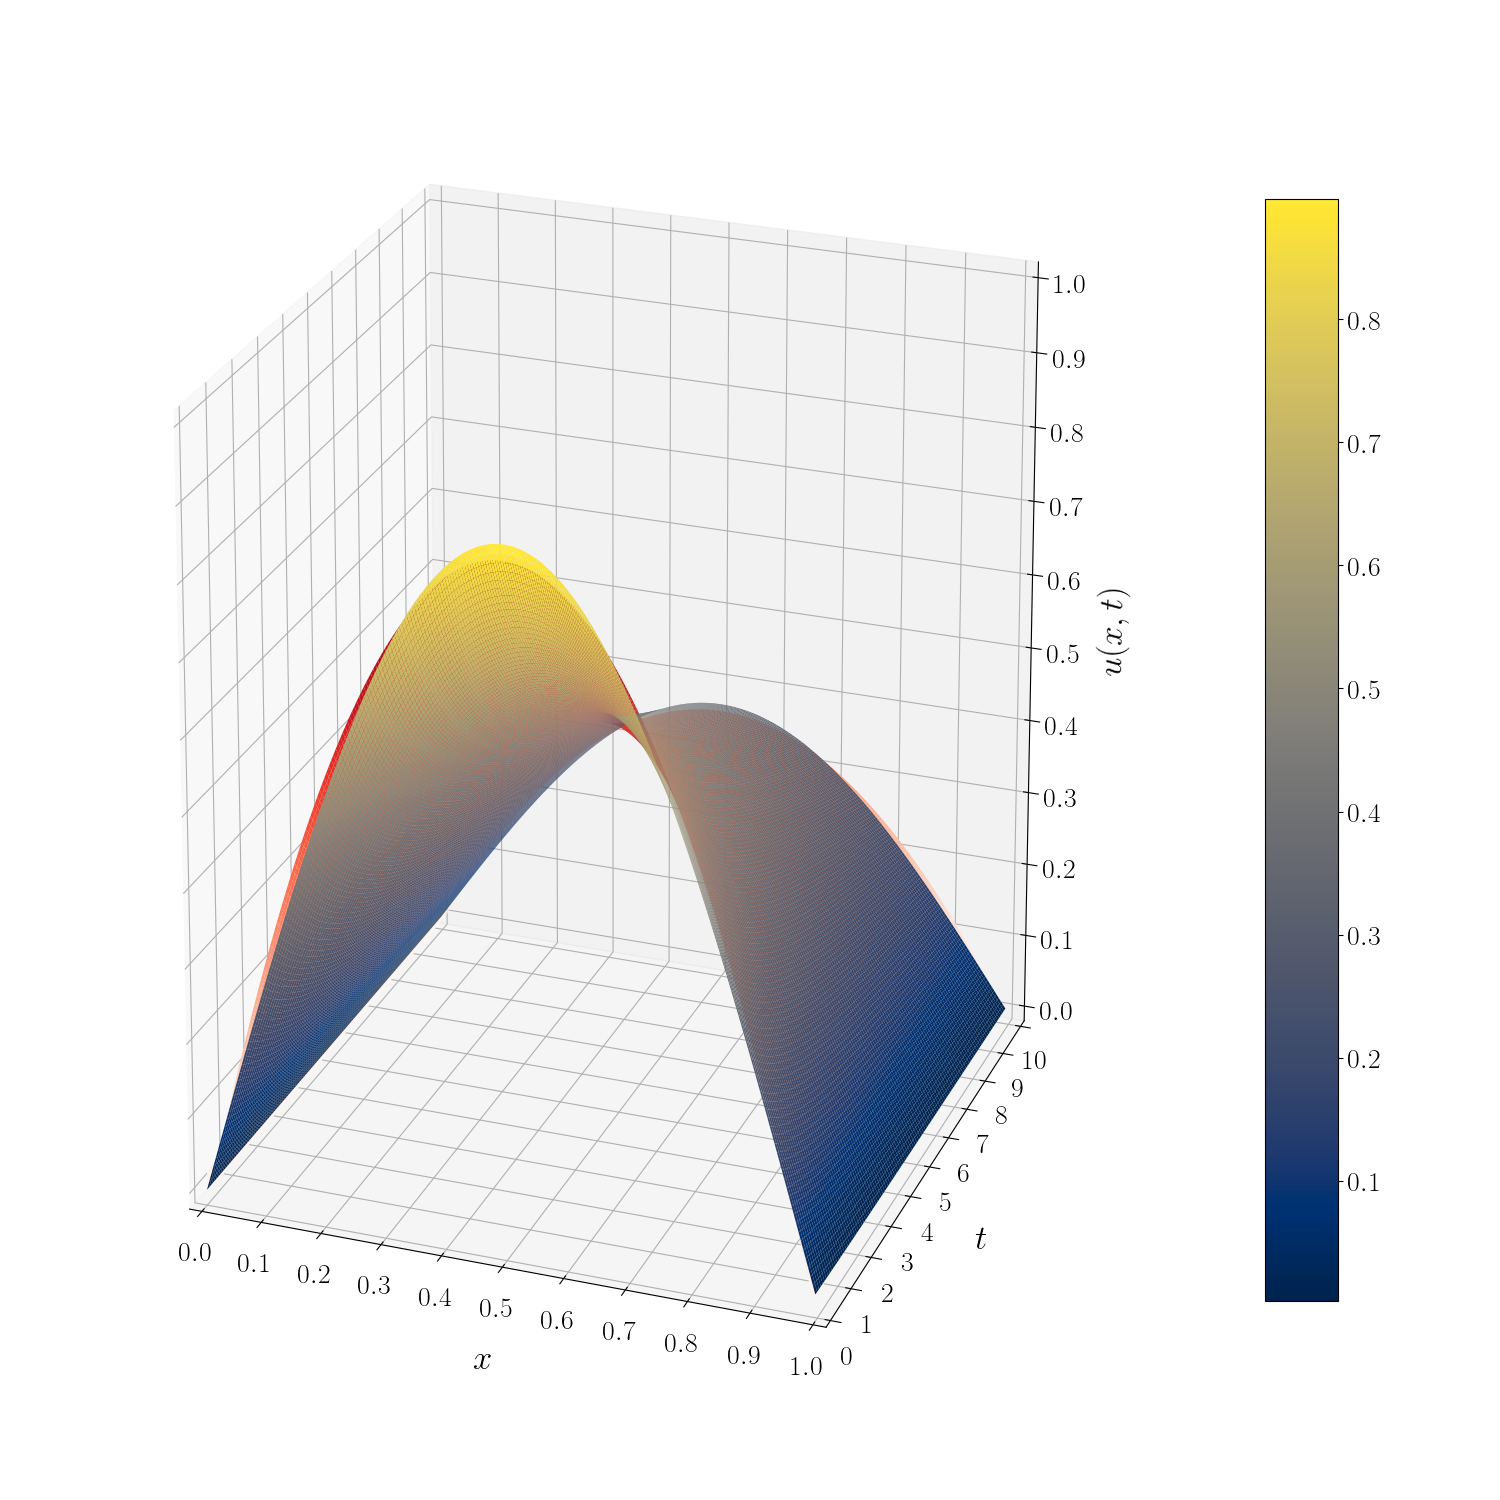
\includegraphics[height=5cm,width=4cm]{files/figures/FPK/Numerical_Solution_Stochastic.png}
	    }
	    \only<2->{
	    \qquad
	    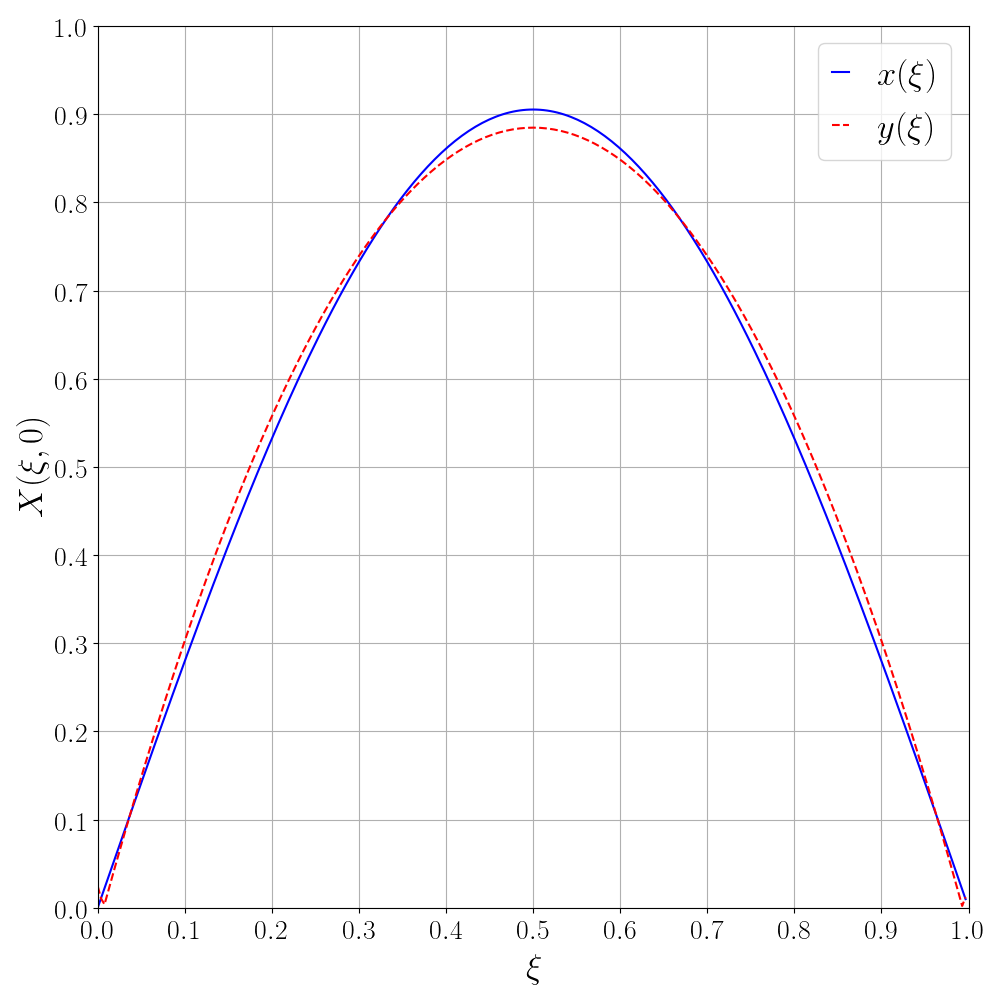
\includegraphics[height=5cm,width=4cm]{files/figures/FPK/IC.png}
    	}
	\end{figure}
\end{frame}

\begin{frame}{Simulaciones: Burgers' Estocastica \hspace{2cm} \hyperlink{Navegador}{\beamergotobutton{Navegador}}}
    \begin{figure}
    \only<1->{
    	\centering
    	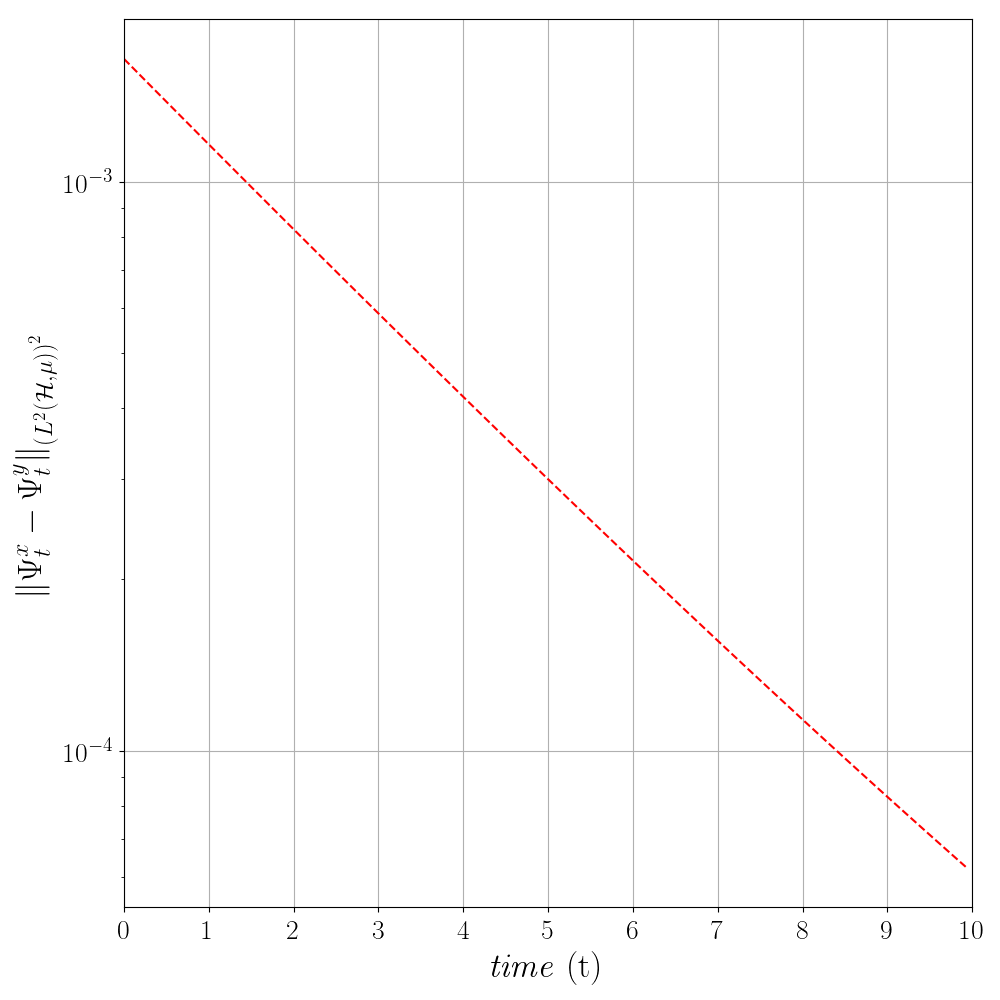
\includegraphics[height=6cm,width=4cm]{files/figures/FPK/norms.png}
    	}
    	\only<2->{
    	\qquad
    	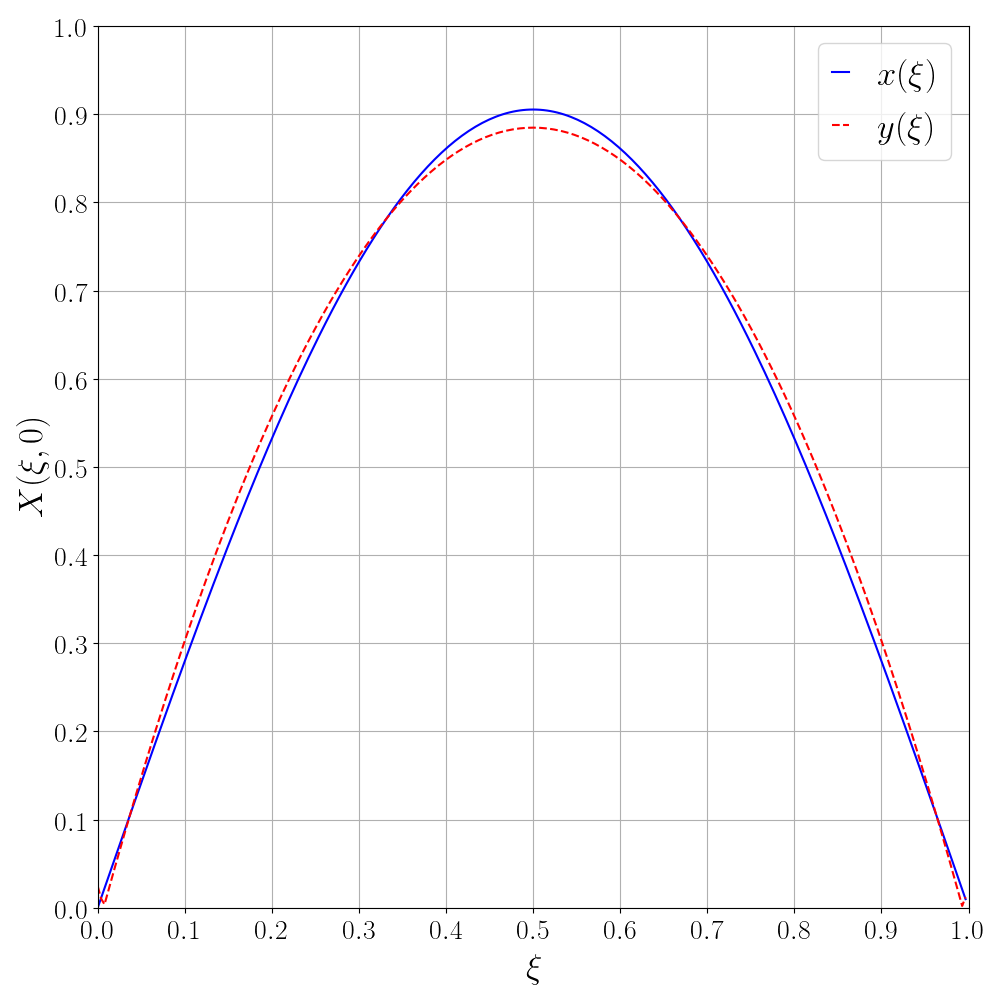
\includegraphics[height=6cm,width=4cm]{files/figures/FPK/IC.png}
    	}
    \end{figure}
\end{frame}	

%=================================================
% end presentation
%=================================================
\end{document}